The governing equations presented in Section \ref{sec:nonlinear continuum electromechanics} are coupled by means of a suitable constitutive law. 
The objective of the following section is to introduce some notions on  constitutive laws in thermo-electro-elasticity. 

\subsection{The Helmholtz free energy}\label{sec:helmholtz}

%\begin{equation}
%\begin{aligned}
%D\vect{F}[\delta\vect{x}] & = \vect{\nabla}_0\delta\vect{x};&\quad
%D^2\vect{F}[\delta\vect{x};\Delta\vect{x}] & = \vect{0};\\
%%
%D\vect{H}[\delta\vect{x}] & = \vect{F}\Cross D\vect{F}[\delta\vect{x}];&\quad
%D^2\vect{H}[\delta\vect{x};\Delta\vect{x}] & =  D\vect{F}[\delta\vect{x}]\Cross D\vect{F}[\Delta\vect{x}];\\
%%
%DJ[\delta\vect{x}] & = \vect{H}:D\vect{F}[\delta\vect{x}];&\quad
%D^2J[\delta\vect{x};\Delta\vect{x}] & = \vect{F}:\left(D\vect{F}[\delta\vect{x}]\Cross D\vect{F}[\Delta\vect{x}]\right).
%\end{aligned}
%\end{equation}


In the case of thermo-electro-elasticity, and in the absence of internal state variables, the Helmholtz free energy $\Psi$ per unit of undeformed volume can be defined as
%
%
\begin{equation}\label{eqn:definition of CMV}
\Psi:\text{GL}^{+}(3)\times \mathbb{R}^3\times \mathbb{R}^+,\qquad \left(\vect{F},\vect{E}_0,\theta\right)\rightarrow \Psi\left(\vect{F},\vect{E}_0,\theta\right)
\end{equation}
%

In order to derive constitutive equations, we begin with the Clausius-Duhen inequality, which takes the following form
%
\begin{equation}\label{eqn:Clausius-Duhen}
-\dot{\Psi} + \vect{P}:\dot{\vect{F}} - \vect{D}_0\cdot \dot{\vect{E}}_0 - \eta \dot{\theta} - \frac{1}{\theta}\vect{Q}\cdot \partial_{\vect{X}}\theta \geq 0
\end{equation}


For the EAP, following \cite{XXX}, use of the Coleman-Noll procedure into \eqref{eqn:Clausius-Duhen}
%
\begin{equation}
\begin{aligned}
\Big(\vect{P} - \partial_{F}\Psi\Big):\dot{\vect{F}} - \Big(\vect{D}_0 + \partial_{\vect{E}_0}\Psi\Big)\cdot \dot{\vect{E}}_0 - \Big(\eta + \partial_{\theta}\Psi\Big) \dot{\theta} - \frac{1}{\theta}\vect{Q}\cdot \partial_{\vect{X}}\theta \geq 0
\end{aligned}	
\end{equation}


Fourier law relates the spatial heat flux $\vect{q}$ and the spatial gradient of $\theta$ by virtue of the following expression
%
\begin{equation}\label{eqn:Duhamel}
\vect{q} = -\vect{k}\partial_{\vect{x}}\theta,
\end{equation}
%
where $\vect{k}$ represents the semi-positive definite second order thermal conductivity tensor in the deformed configuration. The relation between $\vect{q}$ and its material counterpart $\vect{Q}$ in \eqref{eqn:local form energy} can be carried out by making use of the Gauss' theorem and the Nanson's rule (i.e. $d\vect{a}=\vect{H}d\vect{A}$), yielding \cite{XXX}
%
\begin{equation}
\vect{Q} = -\vect{K}\partial_{\vect{X}}\theta;\qquad
\vect{K} = J^{-1}\vect{H}^T\vect{k}\vect{H}.
\end{equation}

Positive definiteness of the material thermal conductivity tensor $\vect{K}$ permits to establish \cite{Gonzalez_book, Gurtin} the following relationships
%
\begin{equation}\label{eqn:first derivatives Hewlmholtz}
\begin{aligned}
\vect{P} = \partial_{F}\Psi(\vect{F},\vect{E}_0,\theta);\qquad  \vect{D}_0 = -\partial_{\vect{E}_0}\Psi(\vect{F},\vect{E}_0,\theta);\qquad  \eta = -\partial_{\theta}\Psi(\vect{F},\vect{E}_0,\theta).
\end{aligned}	
\end{equation}

The Helmholtz free energy density must adhere to the principle of objectivity or material frame indifference, which entails its invariance with repsect to rotations $\vect{Q}\in \text{SO}(3)$ applied to the spatial configuration, namely
%
\begin{equation}\label{eqn:frame indifference}
	\Psi(\vect{Q}\vect{F}, \vect{E}_0, \theta) = \Psi(\vect{F},\vect{E}_0, \theta);\qquad \forall \vect{F}\in \text{GL}^{+}(3),\, \vect{E}_0 \in \mathbb{R}^3,\, \theta \in \mathbb{R}^{+}, \,\vect{Q}\in \text{SO}(3).
\end{equation}

Furthermore, a second invariance condition must hold, known as the material symmetry conditions, which reads as follows
%
\begin{equation}\label{eqn:material symmetry}
	\Psi(\vect{F}\vect{Q}^T,\vect{Q}\vect{E}_0,\theta) = \Psi(\vect{F},\vect{E}_0,\theta);\qquad \forall \vect{F}\in \text{GL}^{+}(3),\, \vect{E}_0 \in \mathbb{R}^3,\,\theta \in \mathbb{R}^{+}, \,\vect{Q}\in \mathcal{G}\subset \text{O}(3),
\end{equation}
%
where $\mathcal{G}$ denotes the symmetry group of the material under consideration.  Section \ref{subsec:InvariantFormulation} will demonstrate how the two physical conditions specified in equation \eqref{eqn:frame indifference} and \eqref{eqn:material symmetry} can be imposed a priori. 
 Moreover, the Helmholtz free energy density $\Psi(\vect{F},\vect{E}_0,\theta)$, along with the first Piola-Kirchhoff stress tensor $\vect{P}(\vect{F},\vect{E}_0,\theta)$, the electric displacement field $\vect{D}_0(\vect{F},\vect{E}_0,\theta)$ and the entropy $\eta(\vect{F},\vect{E}_0,\theta)$ must vanish in the absence of deformations (i.e. $\vect{F}=\vect{I}$, with $\vect{I}$ the second order identity tensor), electric fields (i.e. $\vect{E}_0=\vect{0}$) and when the temperature is equal to the so-called reference temperature, denoted as $\theta_R$. All that is mathematically stated as
%
\begin{equation}\label{eqn:reference conditions}
\begin{aligned}	
\left.\Psi(\vect{F},\vect{E}_0,\theta)\right\vert_{\vect{I},\vect{0},\theta_R}&=0; &\qquad \left.\vect{P}(\vect{F},\vect{E}_0,\theta)\right\vert_{\vect{I},\vect{0},\theta_R}&:=\left.\partial_{\vect{F}}\Psi(\vect{F},\vect{E}_0,\theta)\right\vert_{\vect{I},\vect{0},\theta_R}=\vect{0}\\
%
\left.\vect{D}_0(\vect{F},\vect{E}_0,\theta)\right\vert_{\vect{I},\vect{0},\theta_R}&=:\left.\partial_{\vect{E}_0}\Psi(\vect{F},\vect{E}_0,\theta)\right\vert_{\vect{I},\vect{0},\theta_R}=\vect{0}; &\qquad \left.\eta(\vect{F},\vect{E}_0,\theta)\right\vert_{\vect{I},\vect{0},\theta_R}&:=\left.\partial_{\theta}\Psi(\vect{F},\vect{E}_0,\theta)\right\vert_{\vect{I},\vect{0},\theta_R}={0}
\end{aligned}	
\end{equation}

Equation \eqref{eqn:first derivatives Hewlmholtz} establishes the relationship between the first derivatives of the Helmholtz free energy density, namely $\{\vect{P},\vect{D}_0,\eta\}$, with their work conjugates, namely $\{\vect{F},\vect{E}_0,\theta\}$, thus closing the system of coupled PDEs in \eqref{sec:governing equations}, governing the behaviour of EAPs. However, the second derivatives of the Helmholtz energy lead also to constitutive tensors with insightful physical relevance, in particular when characterizing the behaviour of the EAP in the linearized regime, i.e. in the vicinity of $\vect{F}\approx \vect{I}$, . These can be encompassed within the (symmetric) Hessian of the Helmholtz free energy density, denoted as $[\mathbb{H}_{\Psi}]$, namely
%
\begin{equation}
[\mathbb{H}_{\Psi}]=\begin{bmatrix}
\partial^2_{\vect{F}\vect{F}}\Psi  &  \partial^2_{\vect{F}\vect{E}_0}\Psi  &  \partial^2_{\vect{F}\theta}\Psi\\
%
  &  \partial^2_{\vect{E}_0\vect{E}_0}\Psi  &  \partial^2_{\vect{F}\theta}\Psi\\
%
\text{sym.}  &    &  \partial^2_{\theta\theta}\Psi
\end{bmatrix}
\end{equation}
%
where $\partial^2_{\vect{F}\vect{F}}\Psi$ represents the fourth order elasticity tensor, $\partial^2_{\vect{F}\vect{E}_0}\Psi$ the third order piezoelectric tensor, $\partial^2_{\vect{E}_0\vect{E}_0}\Psi$ represents the second order dielectric tensor, whereas $\partial^2_{\vect{F}\theta}\Psi$ and $\partial^2_{\vect{E}_0\theta}\Psi$ are second and first order tensors encoding the influence of the thermal field $\theta$ on the first Piola-Kirchhoff stress tensor $\vect{P}$ and on the electric displacement field $\vect{D}_0$. Finally, $\partial^2_{\theta\theta}\Psi$ can be related with a relevant physical property of a material, in particular, the specific heat capacity, denoted as $c_v$, and defined as \cite{Vertechhy}
%
\begin{equation}\label{eqn:heat capacity}
c_v(\vect{F},\vect{E}_0,\theta) = -\theta \partial^2_{\theta\theta}\Psi(\vect{F},\vect{E}_0,\theta)
\end{equation}

In addition to the physical conditions encompassing the objectivity condition \eqref{eqn:frame indifference}, the material symmetry condition \eqref{eqn:material symmetry} and the reference conditions \eqref{eqn:reference conditions}, there are mathematical conditions that the Helmholtz free energy density $\Psi(\vect{F},\vect{E}_0,\theta)$ must comply with. In the context of thermo-electro-elasticity, it is accepted that  suitable conditions that $\Psi(\vect{F},\vect{E}_0,\theta)$ must satisfy are: rank-one convexity with respect to the deformation gradient $\vect{F}$, concavity with respect to $\vect{E}_0$, and concavity with respect to the absolute temperature $\theta$, i.e.
%
\begin{equation}\label{eqn:rank one convexity}
\left(\vect{u}\otimes\vect{V}\right):\partial^2_{\vect{F}\vect{F}}\Psi:\left(\vect{u}\otimes\vect{V}\right)\geq 0;\qquad
%
%
%
\begin{bmatrix}
\vect{V}\\
\delta\theta 
\end{bmatrix}: \begin{bmatrix}
\partial^2_{\vect{E}_0\vect{E}_0}\Psi  &  \partial^2_{\vect{E}_0\theta}\Psi\\
%
\text{sym.}  &  \partial^2_{\theta\theta}\Psi
\end{bmatrix}\, \begin{bmatrix}
\vect{V}\\
\delta\theta 
\end{bmatrix}\leq 0,
%
\end{equation}
%
which must hold for $\forall \vect{u},\vect{V}\in \mathbb{R}^{3},\,\delta\theta\in\mathbb{R}^{+}, \,\,\{\vect{F},\vect{E}_0,\theta\}\in\{\text{GL}^{+}(3),\mathbb{R}^3,\mathbb{R}^{+}\}$. Notice that concavity with respect to $\theta$ in \eqref{eqn:rank one convexity} entails positiveness of the specific heat capacity $c_v$ in \eqref{eqn:heat capacity}, whereas the two previous conditions in \eqref{eqn:rank one convexity} are related with the concept of material stability and hyperbolicity in the isothermal case \cite{XX}.


\subsection{Alternative thermodynamical potentials}\label{sec:alternative potentials}

Provided that the Helmholtz free energy density $\Psi(\vect{F},\vect{E}_0,\theta)$ is concave with respect to $\vect{E}_0$ and $\theta$ (as specified by the second and third conditions in \eqref{eqn:rank one convexity}), it becomes possible to define the following three alternative thermodynamic potentials via appropriate Legendre transformations
%
\begin{equation}\label{eqn:other potentials}
\begin{aligned}
e(\vect{F},\vect{D}_0,\eta) & =  \inf_{\vect{E}_0,\theta}\left\{\Psi(\vect{F},\vect{E}_0,\theta) + \vect{E}_0\cdot\vect{D}_0 + \theta \eta \right\}\\
%
\Upsilon(\vect{F},\vect{D}_0,\theta) & =  \inf_{\vect{E}_0}\left\{\Psi(\vect{F},\vect{E}_0,\theta) + \vect{E}_0\cdot\vect{D}_0\right\}\\
%
\Gamma(\vect{F},\vect{E}_0,\eta) & =  \inf_{\theta}\left\{\Psi(\vect{F},\vect{E}_0,\theta) + \theta \eta \right\},
\end{aligned}	
\end{equation}
%
which permits to establish analogous relationships to those in \eqref{eqn:first derivatives Hewlmholtz} as
%
\begin{equation}\label{eqn:piola alternative}
\begin{aligned}
\vect{P}& = \partial_{F}e(\vect{F},\vect{D}_0,\eta);&\qquad  \vect{E}_0& = \partial_{\vect{D}_0}e(\vect{F},\vect{D}_0,\eta);&\qquad  \theta &= \partial_{\eta}e(\vect{F},\vect{D}_0,\eta);\\
%
%
\vect{P} &= \partial_{F}\Upsilon(\vect{F},\vect{D}_0,\theta);&\qquad  \vect{E}_0 &= \partial_{\vect{D}_0}\Upsilon(\vect{F},\vect{D}_0,\theta);&\qquad  \eta &= -\partial_{\theta}\Upsilon(\vect{F},\vect{D}_0,\theta);\\
%
%
\vect{P} &= \partial_{F}\Gamma(\vect{F},\vect{E}_0,\eta);&\qquad  \vect{D}_0& = -\partial_{\vect{E}_0}\Gamma(\vect{F},\vect{E}_0,\eta);&\qquad  \theta& = \partial_{\eta}\Gamma(\vect{F},\vect{E}_0,\eta).
\end{aligned}	
\end{equation} 


Obviously, the three new potentials, $e(\vect{F},\vect{D}_0,\eta)$, $\Upsilon(\vect{F},\vect{D}_0,\theta)$ and $\Gamma(\vect{F},\vect{D}_0,\eta)$ need to comply with the 
material frame indifference condition in \eqref{eqn:frame indifference} and with the material symmetry condition in \eqref{eqn:material symmetry}. Additionally, in the reference configuration, each of these potentials must comply with the conditions below
%
\begin{equation}\label{eqn:reference conditions for the different potentials}
\begin{aligned}
&\left\{\begin{aligned}	
\left.e(\vect{F},\vect{D}_0,\eta)\right\vert_{\vect{I},\vect{0},0}&=0; &\quad \left.{\vect{P}}(\vect{F},\vect{D}_0,\eta)\right\vert_{\vect{I},\vect{0},0}&:=\left.\partial_{\vect{F}}e(\vect{F},\vect{D}_0,\eta)\right\vert_{\vect{I},\vect{0},0}=\vect{0}\\
%
\left.{\vect{E}_0}(\vect{F},\vect{D}_0,\eta)\right\vert_{\vect{I},\vect{0},0}&:=\left.\partial_{\vect{D}_0}e(\vect{F},\vect{D}_0,\eta)\right\vert_{\vect{I},\vect{0},0}=\vect{0}; &\quad \left.\theta(\vect{F},\vect{D}_0,\eta)\right\vert_{\vect{I},\vect{0},0}&:=\left.\partial_{\eta}e(\vect{F},\vect{D}_0,\eta)\right\vert_{\vect{I},\vect{0},0}=\theta_R
\end{aligned}	\right.\\
%
%
&\left\{\begin{aligned}	
\left.\Upsilon(\vect{F},\vect{D}_0,\theta)\right\vert_{\vect{I},\vect{0},\theta_R}&=0; &\quad \left.{\vect{P}}(\vect{F},\vect{D}_0,\theta)\right\vert_{\vect{I},\vect{0},\theta_R}&:=\left.\partial_{\vect{F}}\Upsilon(\vect{F},\vect{D}_0,\theta)\right\vert_{\vect{I},\vect{0},\theta_R}=\vect{0}\\
%
\left.{\vect{E}_0}(\vect{F},\vect{D}_0,\theta)\right\vert_{\vect{I},\vect{0},\theta_R}&:=\left.\partial_{\vect{D}_0}\Upsilon(\vect{F},\vect{D}_0,\theta)\right\vert_{\vect{I},\vect{0},\theta_R}=\vect{0}; &\quad \left.\eta(\vect{F},\vect{D}_0,\theta)\right\vert_{\vect{I},\vect{0},\theta_R}&:=-\left.\partial_{\theta}\Upsilon(\vect{F},\vect{D}_0,\theta)\right\vert_{\vect{I},\vect{0},\theta_R}={0}
\end{aligned}	\right.\\
%
%%
%
&\left\{\begin{aligned}	
\left.\Gamma(\vect{F},\vect{D}_0,\eta)\right\vert_{\vect{I},\vect{0},0}&=0; &\quad \left.{\vect{P}}(\vect{F},\vect{E}_0,\eta)\right\vert_{\vect{I},\vect{0},0}&:=\left.\partial_{\vect{F}}\Gamma(\vect{F},\vect{E}_0,\eta)\right\vert_{\vect{I},\vect{0},0}=\vect{0}\\
%
\left.{\vect{D}_0}(\vect{F},\vect{E}_0,\eta)\right\vert_{\vect{I},\vect{0},0}&:=-\left.\partial_{\vect{D}_0}\Gamma(\vect{F},\vect{E}_0,\eta)\right\vert_{\vect{I},\vect{0},0}=\vect{0}; &\quad \left.\theta(\vect{F},\vect{E}_0,\eta)\right\vert_{\vect{I},\vect{0},0}&:=\left.\partial_{\eta}\Gamma(\vect{F},\vect{E}_0,\eta)\right\vert_{\vect{I},\vect{0},0}=\theta_R
\end{aligned}	\right.\\
%
%
\end{aligned}
\end{equation}



Furthermore, provided that $\Psi(\vect{F},\vect{E}_0,\theta)$ is rank-one convex with respect to $\vect{F}$ (i.e. first condition in \eqref{eqn:rank one convexity}), the resulting thermodynamical potentials in above \eqref{eqn:other potentials} would satisfy the following convexity/concavity properties
%
\begin{equation}\label{eqn:rank one convexity other potentials}
\begin{aligned}
%	
%e(\vect{F},\vect{D}_0,\eta)\Rightarrow 
%
&\begin{bmatrix}
\left(\vect{u}\otimes\vect{V}\right)\\
\vect{V}_{\perp}\\
\delta \eta
\end{bmatrix}:\begin{bmatrix}
\partial^2_{\vect{F}\vect{F}}e  &  \partial^2_{\vect{F}\vect{D}_0}e  &  \partial^2_{\vect{F}\eta}e\\
%
\partial^2_{\vect{F}\vect{F}}e  &  \partial^2_{\vect{F}\vect{D}_0}e  &  \partial^2_{\vect{F}\eta}e\\
%
\partial^2_{\vect{F}\vect{F}}e  &  \partial^2_{\vect{F}\vect{D}_0}e  &  \partial^2_{\vect{F}\eta}e
\end{bmatrix}:\begin{bmatrix}
\left(\vect{u}\otimes\vect{V}\right)\\
\vect{V}_{\perp}\\
\delta \eta
\end{bmatrix}
\geq 0;&\\
%
%
%
%\Upsilon(\vect{F},\vect{D}_0,\theta)\Rightarrow 
%
&\begin{bmatrix}
\left(\vect{u}\otimes\vect{V}\right)\\
\vect{V}_{\perp}
\end{bmatrix}:\begin{bmatrix}
\partial^2_{\vect{F}\vect{F}}\Upsilon  &  \partial^2_{\vect{F}\vect{D}_0}\Upsilon  \\
%
\text{sym.}  &  \partial^2_{\vect{D}_0\vect{D}_0}\Upsilon\\
\end{bmatrix}:\begin{bmatrix}
\left(\vect{u}\otimes\vect{V}\right)\\
\vect{V}_{\perp}
\end{bmatrix}
\geq 0;&\qquad
%
%
&\partial^2_{\theta\theta}\Upsilon\leq 0;\\
%
%
%
%\Gamma(\vect{F},\vect{E}_0,\eta)\Rightarrow 
%
&\begin{bmatrix}
\left(\vect{u}\otimes\vect{V}\right)\\
\delta \eta
\end{bmatrix}:\begin{bmatrix}
\partial^2_{\vect{F}\vect{F}}\Gamma   &  \partial^2_{\vect{F}\eta}\Gamma\\
%
\text{sym.} & \partial^2_{\eta\eta}\Gamma
\end{bmatrix}:\begin{bmatrix}
\left(\vect{u}\otimes\vect{V}\right)\\
\delta \eta
\end{bmatrix}
\geq 0;&\qquad
%
&\vect{V}\cdot \partial^2_{\vect{E}_0\vect{E}_0}\Gamma\, \vect{V}\geq 0,
%
%
\end{aligned}
\end{equation}
%
%
%
%
which must hold for 
%
\begin{equation}
\begin{aligned}
& \vect{u},\vect{V},\vect{V}_{\perp}
\in \mathbb{R}^{3}, \delta\eta\in\mathbb{R},&\quad&\{\vect{F},\vect{D}_0,\eta\}\in\{\text{GL}^{+}(3),\mathbb{R}^3,\mathbb{R}\}	\\
 %
&\vect{u},\vect{V},\vect{V}_{\perp}\in \mathbb{R}^{3},&\quad&\{\vect{F},\vect{D}_0,\theta\}\in\{\text{GL}^{+}(3),\mathbb{R}^3,\mathbb{R}^{+}\}\\
%
&\vect{u},\vect{V}\in \mathbb{R}^{3}, \delta\eta\in\mathbb{R},&\quad&\{\vect{F},\vect{E}_0,\eta\}\in\{\text{GL}^{+}(3),\mathbb{R}^3,\mathbb{R}\},		 
\end{aligned}	
\end{equation}
%
%
respectively, where $\vect{V}_{\perp}$ is such that $\vect{V}_{\perp}\cdot \vect{V}=0$. Above conditions, in conjunction with \eqref{eqn:rank one convexity} dictate that the four potentials, namely $\Psi(\vect{F},\vect{E}_0,\theta)$, $e(\vect{F},\vect{D}_0,\eta)$, $\Upsilon(\vect{F},\vect{D}_0,\theta)$ and $\Gamma(\vect{F},\vect{E}_0,\theta)$, in the vicinity of the reference configuration, namely $\vect{F}\approx \vect{I}$, $\vect{E}_0\approx \vect{0}$ and $\theta\approx \theta_R$, will adopt the convexity/concavity properties displayed in Figure \eqref{fig:convexity}.

\begin{figure}[htpb!]	
	\centering
	\begin{tabular}{cc}
	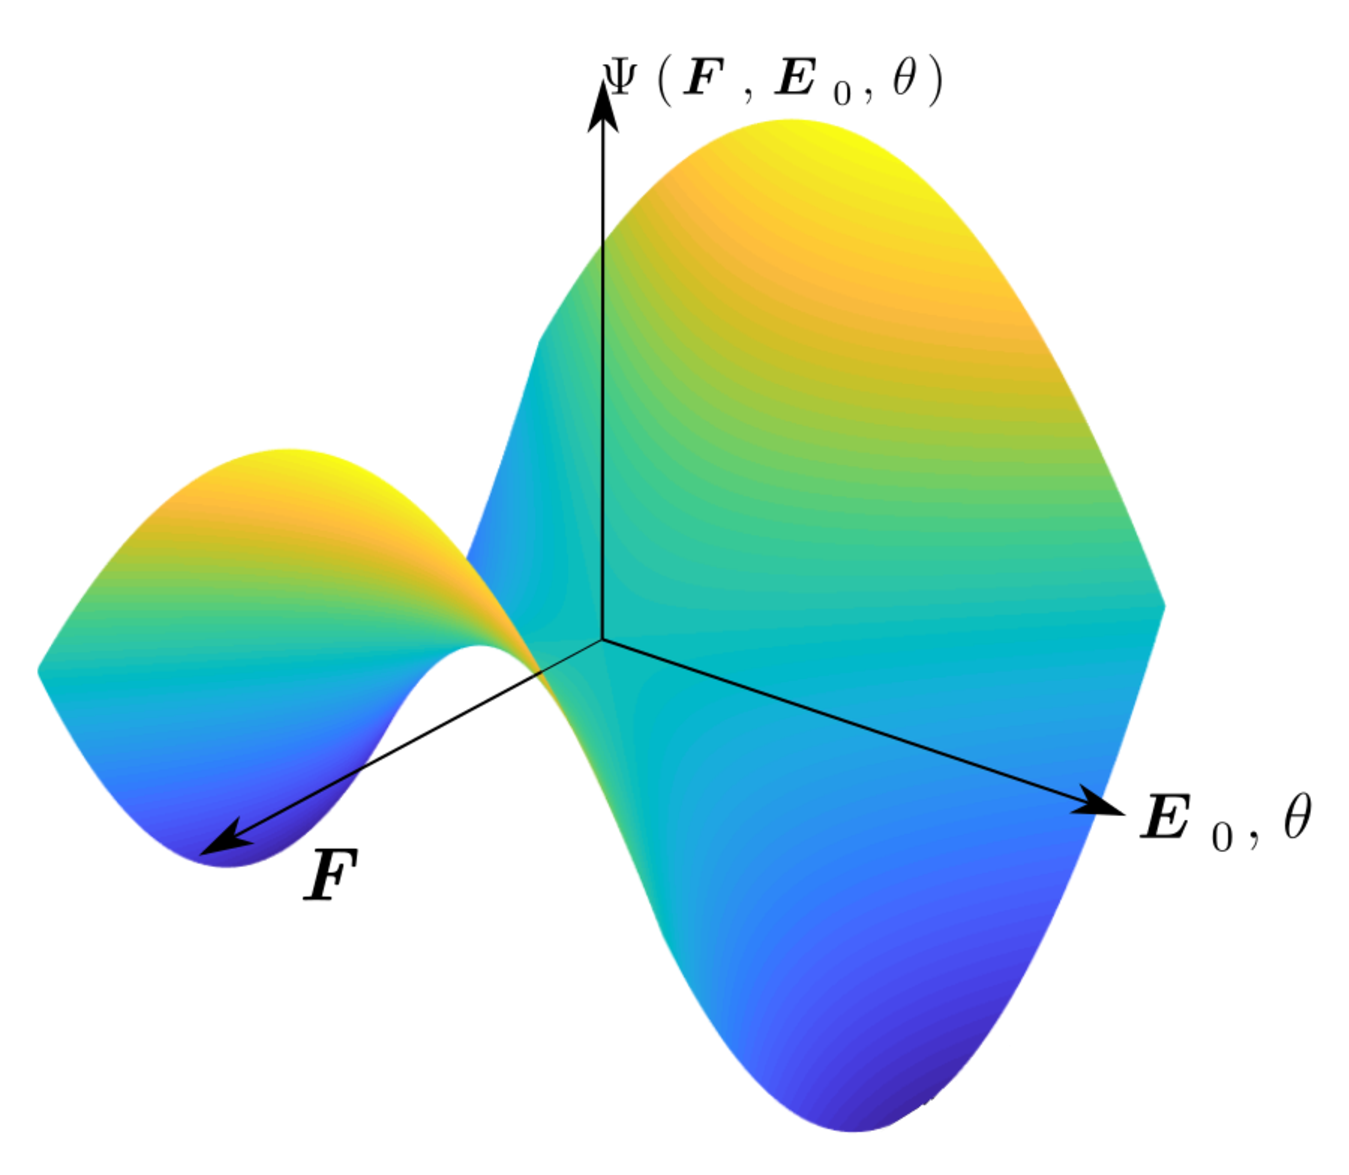
\includegraphics[width=0.35\textwidth]{Figures/InkScape/convexity_psi}&
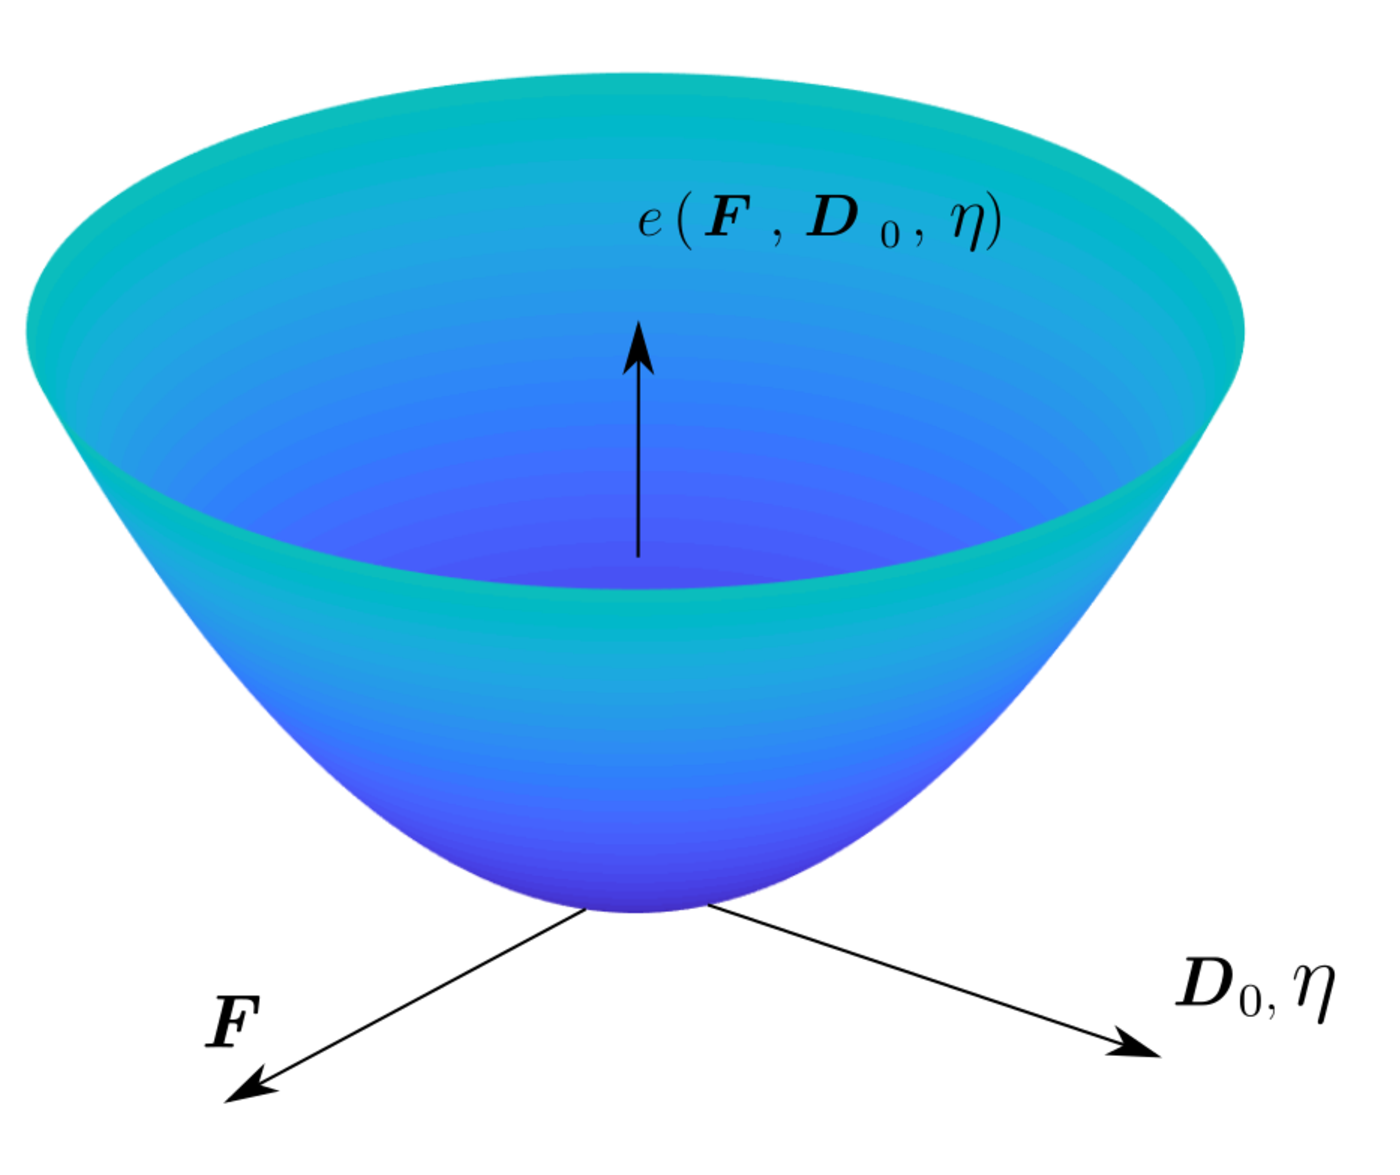
\includegraphics[width=0.35\textwidth]{Figures/InkScape/convexity_e}\\
%
(a)  &  (b)\\
%
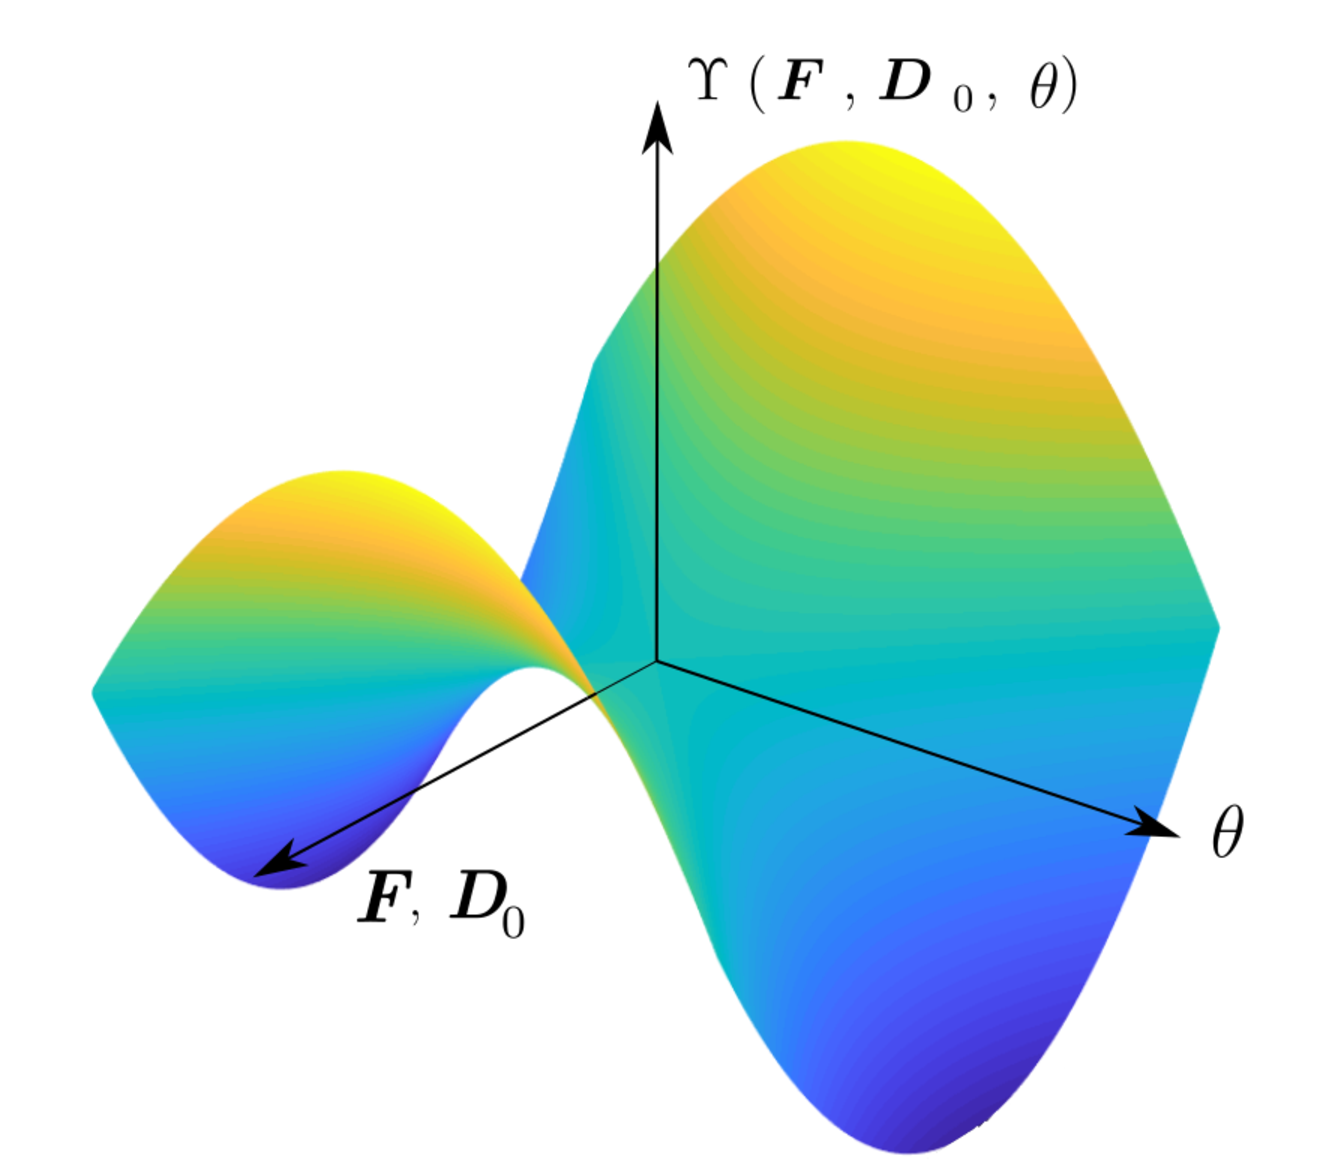
\includegraphics[width=0.35\textwidth]{Figures/InkScape/convexity_upsilon}&
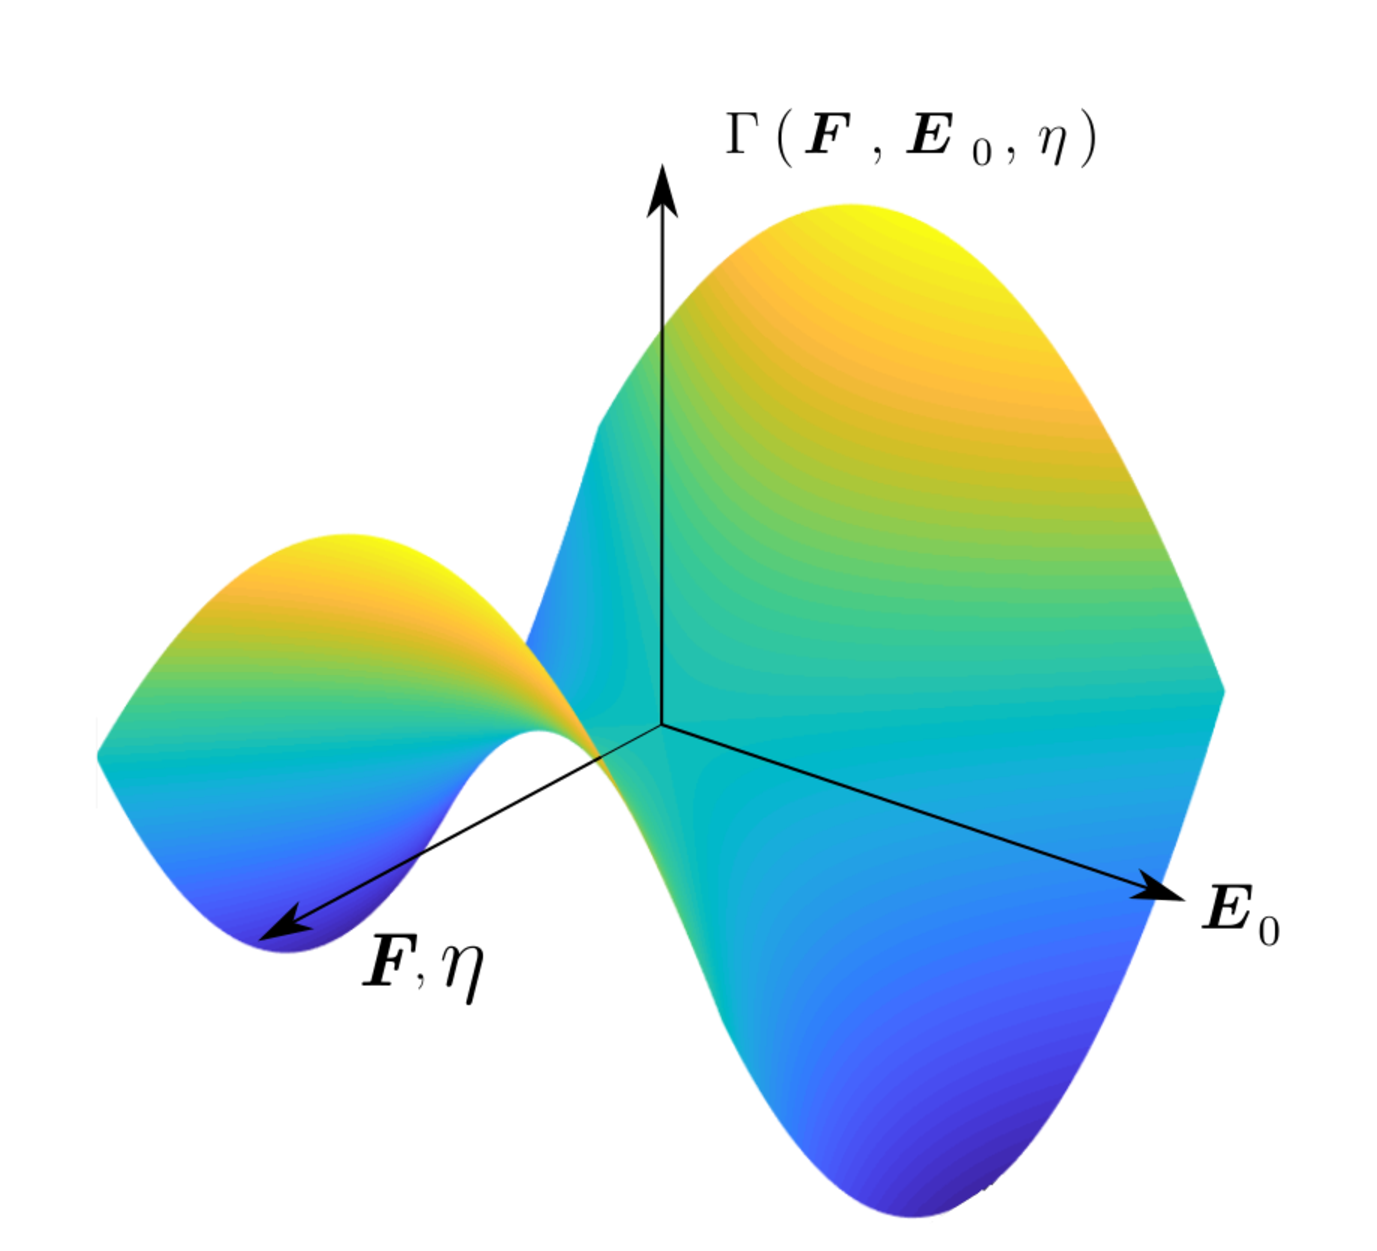
\includegraphics[width=0.35\textwidth]{Figures/InkScape/convexity_gamma}	\\
%	
(c)  &  (d)
	\end{tabular}
	\vspace{-2mm}
	\caption{Convexity/concavity properties of the various thermodynamical potentials $\Psi(\vect{F},\vect{E}_0,\theta)$, $e(\vect{F},\vect{D}_0,\eta)$, $\Upsilon(\vect{F},\vect{D}_0,\theta)$ and $\Gamma(\vect{F},\vect{E}_0,\theta)$ in the vicinity of the reference configuration (i.e. $\vect{F}\approx \vect{I}$, $\vect{E}_0\approx \vect{0}$ and $\theta\approx \theta_R$). Specifically, we observe: $\Psi(\vect{F},\vect{E}_0,\theta)$ is convex with respect to $\vect{F}$ and concave with respect to $\{\vect{E}_0,\theta\}$; $e(\vect{F},\vect{D}_0,\eta)$ is convex with respect to $\{\vect{F},\vect{D}_0,\eta\}$; $\Upsilon(\vect{F},\vect{D}_0,\theta)$ is convex with respect to $\{\vect{F},\vect{D}_0\}$ and concave with respect to $\theta$; $\Gamma(\vect{F},\vect{E}_0,\eta)$ is convex with respect to $\{\vect{F},\eta\}$ and concave with respect to $\vect{E}_0$.}
	\label{fig:convexity}
\end{figure}

 
 
 


As discussed in \cite{XX}, defining phenomenological thermodynamic potentials that must satisfy both rank-one convexity and concavity conditions-such as $\Psi(\vect{F},\vect{E}_0,\theta)$, $\Upsilon(\vect{F},\vect{D}_0,\theta)$, and $\Gamma(\vect{F},\vect{E}_0,\eta)$-is generally more challenging than when the potential is only required to be rank-one convex or convex with respect to all its arguments, as is the case with the internal energy $e(\vect{F},\vect{D}_0,\theta)$. Motivated by this simplification, the authors in \cite{XX} aimed to define constitutive models for the internal energy of EAPs within the framework of isothermal electro-mechanics. This was achieved by extending the concept of polyconvexity, originally from hyperelasticity (purely mechanical systems), to this multi-physics context. Indeed, a sufficient condition for ensuring the rank-one convexity of $e(\vect{F},\vect{D}_0,\eta)$, as shown in equation \eqref{eqn:rank one convexity other potentials}, can be fulfilled through the polyconvexity of $e(\vect{F},\vect{D}_0,\eta)$. For this purpose, we assume the existence of a function $\mathbb{W}$ such that:
%
\begin{equation}
\mathbb{W}:\text{GL}^{+}(3)\times \text{GL}^{+}(3)\times \mathbb{R}^{+}\times \mathbb{R}^3\times \mathbb{R}^3\times \mathbb{R},\qquad (\vect{F},\vect{H},J,\vect{D}_0,\vect{d},\eta)\rightarrow \mathbb{W}(\vect{F},\vect{H},J,\vect{D}_0,\vect{d},\eta)
\end{equation}
%
where $\vect{H}$ and $J$ are the co-factor and determinant of $\vect{F}$, defined in \eqref{eqn:H and J classical} and \eqref{eqn:H and J tensor cross product expression}, whilst $\vect{d}$ is a field obtained as $\vect{d}=\vect{FD}_0$. Then, $e(\vect{F},\vect{D}_0,\eta)$ is said to be polyconvex \cite{Ball_1976,Ball_2002,Ball_Murat_1976} if it can be equivalently written as
%
\begin{equation}\label{eqn:polyconvexity}
e(\vect{F},\vect{D}_0,\eta)=\mathbb{W}(\vect{F},\vect{H},J,\vect{D}_0,\vect{d},\eta)
\end{equation}
%
where $\mathbb{W}(\vect{F},\vect{H},J,\vect{D}_0,\vect{d},\eta)$ must be convex with respect to all its arguments. For twicely differentiable functions, convexity of $\mathbb{W}(\vect{F},\vect{H},J,\vect{D}_0,\vect{d},\eta)$ is equivalent to positive definiteness of its Hessian operator $[\mathbb{H}_{\mathbb{W}}]$, i.e.
%
\begin{equation}
\delta{\mathcal{V}}^T:[\mathbb{H}_{\mathbb{W}}]:\delta{\mathcal{V}}\geq 0,\quad \forall\, \delta\mathcal{V}=\begin{bmatrix}\delta\vect{F} & \delta\vect{H} & \delta J & \delta\vect{D}_0 & \delta\vect{d} & \delta \eta
\end{bmatrix}^T,
\end{equation}
%
where the (symmetric) Hessian operator  $[\mathbb{H}_{\mathbb{W}}]$ incorporates all the second derivatives of $\mathbb{W}$, i.e.
%
\begin{equation}
[\mathbb{H}_{\mathbb{W}}]=\begin{bmatrix}
\partial^2_{\vect{F}\vect{F}}\mathbb{W}  &  
\partial^2_{\vect{F}\vect{H}}\mathbb{W}  &
\partial^2_{\vect{F}J}\mathbb{W}&
\partial^2_{\vect{F}\vect{D}_0}\mathbb{W}&
\partial^2_{\vect{F}\vect{d}}\mathbb{W}&
\partial^2_{\vect{F}\eta}\mathbb{W}\\
%
%
&
\partial^2_{\vect{H}\vect{H}}\mathbb{W}  &
\partial^2_{\vect{H}J}\mathbb{W}&
\partial^2_{\vect{H}\vect{D}_0}\mathbb{W}&
\partial^2_{\vect{H}\vect{d}}\mathbb{W}&
\partial^2_{\vect{H}\eta}\mathbb{W}\\
%
%
& &
\partial^2_{JJ}\mathbb{W}&
\partial^2_{J\vect{D}_0}\mathbb{W}&
\partial^2_{J\vect{d}}\mathbb{W}&
\partial^2_{J\eta}\mathbb{W}\\
%
%
&&&\partial^2_{\vect{D}_0\vect{D}_0}\mathbb{W}&
\partial^2_{\vect{D}_0\vect{d}}\mathbb{W}&
\partial^2_{\vect{D}_0\eta}\mathbb{W}\\
%
%
\text{sym.}&&&&\partial^2_{\vect{d}\vect{d}}\mathbb{W}&
\partial^2_{\vect{d}\eta}\mathbb{W}\\
%
%
&&&&&\partial^2_{\eta\eta}\mathbb{W}
%
\end{bmatrix}
\end{equation}



\subsection{Invariant-based thermo-electro-mechanics}\label{subsec:InvariantFormulation}


A simple manner to accommodate the principle of objectivity or material frame indifference and the requirement of material symmetry is through the dependence of any of the thermodynamical potentials, namely $\Psi(\vect{F},\vect{E}_0,\theta)$, $e(\vect{F},\vect{D}_0,\eta)$, $\Upsilon(\vect{F},\vect{D}_0,\theta)$ or $\Gamma(\vect{F},\vect{E}_0,\eta)$
with respect to invariants of the right Cauchy-Green deformation gradient tensor $\vect{C}=\vect{F}^T\vect{F}$,  $\vect{E}_0$ or $\vect{D}_0$ and also with respect to $\theta$ or $\eta$. Let us denote as  ${\bf I}_{\Psi}$, ${\bf I}_{e}$, ${\bf I}_{\Upsilon}$ and ${\bf I}_{\Gamma}$ the set of electro-mechanical objective invariants of $\Psi(\vect{F},\vect{E}_0,\theta)$, $e(\vect{F},\vect{D}_0,\eta)$, $\Upsilon(\vect{F},\vect{D}_0,\theta)$ or $\Gamma(\vect{F},\vect{E}_0,\eta)$, respectively,  required to characterise a given material symmetry group $\mathcal{G}$. Then, it is possible to express the four thermodynamical potentials equivalently as
%
\begin{equation}\label{eqn:Energy_wrt_Invariants}
\begin{aligned}
% 	U:\mathbb{R}^n\rightarrow \mathbb{R},\qquad (\vect{\mathcal{I}})\mapsto
% U({\bf I}),\qquad 
\Psi(\vect{F},\vect{E}_0,\theta)&=\mathbb{U}_{\Psi}({\bf I}_{\Psi}(\vect{C},\vect{E}_0),\theta);&\qquad
%
e(\vect{F},\vect{D}_0,\eta)&=\mathbb{U}_{e}({\bf I}_{e}(\vect{C},\vect{D}_0),\eta);\\
%
\Upsilon(\vect{F},\vect{D}_0,\theta)&=\mathbb{U}_{\Upsilon}({\bf I}_{\Upsilon}(\vect{C},\vect{D}_0),\theta);&\qquad
%
\Gamma(\vect{F},\vect{E}_0,\eta)&=\mathbb{U}_{\Gamma}({\bf I}_{\Gamma}(\vect{C},\vect{E}_0),\eta).
%
\end{aligned}
\end{equation}

Application of the chain rule into equation \eqref{eqn:first derivatives Hewlmholtz} or \eqref{eqn:piola alternative} permits of obtain the first Piola-Kirchhoff stress tensor $\vect{P}$, $\vect{D}_0$ or $\vect{E}_0$, and $\theta$ or $\eta$ in terms of the derivatives of above invariant-based potentials with respect to their arguments
%
\begin{equation}\label{eqn:Piola invariants isotropy}
\begin{aligned}	
\vect{P}&=\sum_{i=1}^n\Big(\partial_{I_{\Psi_i}}\mathbb{U}_{\Psi}\Big) \partial_{\vect{F}}I_{\Psi_i};&\qquad
%
\vect{D}_0&=-\sum_{i=1}^n\Big(\partial_{I_{\Psi_i}}\mathbb{U}_{\Psi}\Big) \partial_{\vect{E}_0}I_{\Psi_i};&\qquad
%
\eta  & =  -\partial_\theta \mathbb{U}_{\Psi}\\
%
%
\vect{P}&=\sum_{i=1}^n\Big(\partial_{I_{e_i}}\mathbb{U}_e\Big) \partial_{\vect{F}}I_{e_i};&\qquad
%
\vect{E}_0&=\sum_{i=1}^n\Big(\partial_{I_{e_i}}\mathbb{U}_e\Big) \partial_{\vect{D}_0}I_{e_i};&\qquad
%
\theta &  =  \partial_\eta \mathbb{U}_e\\
%
%
\vect{P}&=\sum_{i=1}^n\Big(\partial_{I_{\Upsilon_i}}\mathbb{U}_{\Upsilon}\Big) \partial_{\vect{F}}I_{\Upsilon_i};&\qquad
%
\vect{E}_0&=\sum_{i=1}^n\Big(\partial_{I_{\Upsilon_i}}\mathbb{U}_{\Upsilon}\Big) \partial_{\vect{D}_0}I_{\Upsilon_i};&\qquad
%
\eta &  =  -\partial_\theta \mathbb{U}_{\Upsilon}\\
%
%
\vect{P}&=\sum_{i=1}^n\Big(\partial_{I_{\Psi_i}}\mathbb{U}\Big) \partial_{\vect{F}}I_{\Psi_i};&\qquad
%
\vect{D}_0&=-\sum_{i=1}^n\Big(\partial_{I_{{\Gamma}_i}}\mathbb{U}_{\Gamma}\Big) \partial_{\vect{E}_0}I_{{\Gamma}_i};&\qquad
%
\theta  & =  \partial_\eta \mathbb{U}_{\Gamma}
%
\end{aligned}
\end{equation}

%Furthermore, application of the chain rule over equation \eqref{eqn:elasticity} permits to obtain the elasticity tensor $\vect{\mathcal{C}}$ in terms of the derivatives of $U({\bf I})$ as
%
%\begin{equation}\label{eqn:elasticity invariants}
%	\vect{\mathcal{C}}=\sum_{i=1}^n\sum_{j=1}^n\left(\partial^2_{I_iI_j}U\right)\partial_{\vect{F}}I_i\otimes\partial_{\vect{F}}I_j + \sum_{i=1}^n\left(\partial_{I_i}U\right)\partial^2_{\vect{F}\vect{F}}I_i.
%\end{equation}



\subsubsection{Electro-mechanical invariants for isotropy}

For the case of isotropy, the invariants required to characterise this material symmetry group for the thermodynamical potentials depending on $\vect{E}_0$, namely $\Psi(\vect{F},\vect{E}_0,\theta)$ and $\Gamma(\vect{F},\vect{E}_0,\eta)$, and the first derivatives of the latter with respect to $\vect{F}$ and $\vect{E}_0$ (featuring in the definition of $\vect{P}$ and $\vect{D}_0$ in \eqref{eqn:Piola invariants isotropy}) are
%
\begin{equation}\label{eqn:table isotropy}
\begin{aligned}	
I_{\Psi_1} &:= \vect{F}:\vect{F}=\text{tr}(\vect{C}),\quad   &\partial_{\vect{F}}I_{\Psi_1}&=2\vect{F},\quad   &\partial_{\vect{D}_0}I_{\Psi_1}&=\vect{0}\\
%
I_{\Psi_2} &:= \vect{H}:\vect{H}=\text{tr}(\text{Cof}\vect{C}),\quad   &\partial_{\vect{F}}I_{\Psi_2}&=2\vect{H}\Cross \vect{F},\quad   &\partial_{\vect{E}_0}I_{\Psi_2}&=\vect{0}\\
%
I_{\Psi_3}&:=J = (\text{det}\vect{C})^{1/2},&\quad   \partial_{\vect{F}}I_{\Psi_3}&=\vect{H},\quad   &\partial_{\vect{D}_0}I_{\Psi_3}&=0\\
%
I_{\Psi_4} &:= \vect{E}_0\cdot\vect{E}_0,\quad   &\partial_{\vect{F}}I_{\Psi_4}&=\vect{0},\quad   &\partial_{\vect{E}_0}I_{\Psi_4}&=2\vect{E}_0\\
%
I_{\Psi_5} &:= \vect{HE}_0\cdot \vect{HE}_0=\vect{E}_0\cdot \text{Cof}\vect{C}\vect{E}_0,\quad   &\partial_{\vect{F}}I_{\Psi_5}&=\Big(2\vect{H}\vect{E}_0\otimes\vect{E}_0\Big)\Cross\vect{F},\quad   &\partial_{\vect{E}_0}I_{\Psi_5}&=2\text{Cof}\vect{C}\vect{E}_0
%		
\end{aligned}
\end{equation}
%
with $I_{\Psi_i}=I_{\Gamma_i}$, for $i=\{1,\dots,5\}$. On the other hand, for the thermodynamical potentials depending on $\vect{D}_0$, namely $e(\vect{F},\vect{D}_0,\eta)$ and $\Upsilon(\vect{F},\vect{D}_0,\theta)$, the invariants and their first derivatives with respect to $\vect{F}$ and $\vect{D}_0$ (featuring in the definition of $\vect{P}$ and $\vect{E}_0$ in \eqref{eqn:Piola invariants isotropy}) have been chosen to be
%
\begin{equation}\label{eqn:table isotropy 2}
\begin{aligned}	
I_{e_1} &:= \vect{F}:\vect{F}=\text{tr}(\vect{C}),\qquad   &\partial_{\vect{F}}I_{e_1}&=2\vect{F},\qquad   &\partial_{\vect{D}_0}I_{e_1}&=\vect{0}\\
%
I_{e_2} &:= \vect{H}:\vect{H}=\text{tr}(\text{Cof}\vect{C}),\qquad   &\partial_{\vect{F}}I_{e_2}&=2\vect{H}\Cross \vect{F},\qquad   &\partial_{\vect{D}_0}I_{e_2}&=\vect{0}\\
%
I_{e_3}&:=J = (\text{det}\vect{C})^{1/2},&\qquad   \partial_{\vect{F}}I_{e_3}&=\vect{H},\qquad   &\partial_{\vect{D}_0}I_{e_3}&=0\\
%
I_{e_4} &:= \vect{D}_0\cdot\vect{D}_0,\qquad   &\partial_{\vect{F}}I_{e_4}&=\vect{0},\qquad   &\partial_{\vect{D}_0}I_{e_4}&=2\vect{D}_0\\
%
I_{e_5} &:= \vect{FD}_0\cdot \vect{FD}_0=\vect{D}_0\cdot \vect{C}\vect{D}_0,\qquad   &\partial_{\vect{F}}I_{e_5}&=2\vect{F}\vect{D}_0\otimes\vect{D}_0,\qquad   &\partial_{\vect{D}_0}I_{e_5}&=2\vect{C}\vect{D}_0,
%		
\end{aligned}
\end{equation}
%
with $I_{e_i}=I_{\Upsilon_i}$, for $i=\{1,\dots,5\}$.



\subsubsection{Electro-mechanical invariants for transversely isotropy}

In the context of transverse isotropy, a preferred direction $\vect{N}$ emerges, perpendicular to the material's plane of isotropy, imparting anisotropic characteristics. Our focus centers on the material symmetry group $\mathcal{D}_{\infty h}$ \cite{HORAK_electro}, where the structural tensor takes the form $\vect{N}\otimes\vect{N}$. This group is distinct from $\mathcal{C}_{\infty}$, also present in transversely isotropic materials, characterized by the structural vector $\vect{N}$ and encompassing the potential for piezoelectricity. The $\mathcal{D}_{\infty h}$ group, beyond the invariants $\{I_1,I_2,I_3,I_4,I_5\}$ in \eqref{eqn:table isotropy}, is distinguished by three additional invariants, which for the case of the thermodynamical potentials $\Psi(\vect{F},\vect{E}_0,\theta)$ and $\Gamma(\vect{F},\vect{E}_0,\eta)$ are detailed below
%
\begin{equation}\label{eqn:TI}
\begin{aligned}	
%
&I_{\Psi_6}=\vect{F}\vect{N}\cdot\vect{F}\vect{N}=\text{tr}\left(\vect{C}\vect{N}\otimes\vect{C}\right),&\quad &\partial_{\vect{F}}I_{\Psi_6}=2\vect{F}\vect{N}\otimes\vect{N},&\quad &\partial_{\vect{E}_0}I_{\Psi_6}=\vect{0}\\
%
%
&I_{\Psi_7}=\vect{H}\vect{N}\cdot\vect{H}\vect{N}=\text{tr}(\text{Cof}\vect{C})
%
%
,&\quad   
&\partial_{\vect{F}}I_{\Psi_7}=2\left(\vect{H}\vect{N}\otimes\vect{N}\right)\Cross \vect{F},&\quad &\partial_{\vect{E}_0}I_{\Psi_7}=\vect{0}\\
%
%
&I_{\Psi_8}=\left(\vect{E}_0\cdot\vect{N}\right)^2
%
%
,&\quad   
&\partial_{\vect{F}}I_{\Psi_8}=\vect{0},&\quad &\partial_{\vect{E}_0}I_{\Psi_8}=2(\vect{E}_0\cdot \vect{N})\vect{N},
%
\end{aligned}
\end{equation}
%
with $I_{\Psi_i}=I_{\Gamma_i}$, for $i=\{1,\dots,8\}$. On the other hand, for the thermodynamical potentials depending on $\vect{D}_0$, namely $e(\vect{F},\vect{D}_0,\eta)$ and $\Upsilon(\vect{F},\vect{D}_0,\theta)$, the invariants and their first derivatives with respect to $\vect{F}$ and $\vect{D}_0$ (featuring in the definition of $\vect{P}$ and $\vect{E}_0$ in \eqref{eqn:Piola invariants isotropy}), in addition to those in \eqref{eqn:table isotropy 2}, have been chosen to be
%
\begin{equation}\label{eqn:TI 2}
\begin{aligned}	
%
&I_{\Psi_6}=\vect{F}\vect{N}\cdot\vect{F}\vect{N}=\text{tr}\left(\vect{C}\vect{N}\otimes\vect{C}\right),&\quad &\partial_{\vect{F}}I_{\Psi_6}=2\vect{F}\vect{N}\otimes\vect{N},&\quad &\partial_{\vect{D}_0}I_{\Psi_6}=\vect{0}\\
%
%
&I_{\Psi_7}=\vect{H}\vect{N}\cdot\vect{H}\vect{N}=\text{tr}(\text{Cof}\vect{C})
%
%
,&\quad   
&\partial_{\vect{F}}I_{\Psi_7}=2\left(\vect{H}\vect{N}\otimes\vect{N}\right)\Cross \vect{F},&\quad &\partial_{\vect{D}_0}I_{\Psi_7}=\vect{0}\\
%
%
&I_{\Psi_8}=\left(\vect{D}_0\cdot\vect{N}\right)^2
%
%
,&\quad   
&\partial_{\vect{F}}I_{\Psi_8}=\vect{0},&\quad &\partial_{\vect{D}_0}I_{\Psi_8}=2(\vect{D}_0\cdot \vect{N})\vect{N},
%
\end{aligned}
\end{equation}
%
with $I_{e_i}=I_{\Upsilon_i}$, for $i=\{1,\dots,8\}$.


\subsection{The ground truth thermo-electro-mechanical Helmholtz free energy free density}\label{sec:ground truth model}

In this study, we will calibrate our neural network-based constitutive models using a series of in-silico datasets derived from various ground truth constitutive models. Each of these models will be formulated based on a Helmholtz free energy density that shares a common structural framework, as established by the seminal work of XX in the domain of thermomechanics, and further extended by XX in the context of thermo-electromechanics. Consequently, all ground truth models will be defined in accordance with the following decomposition:
%
\begin{equation}\label{eqn:additive decomposition}
\begin{aligned}
\Psi\left(\vect{F},\vect{E}_0,\theta\right)& = \mathcal{F}(\theta)\Big({\Psi}_{m}\left(\vect{F}\right)+{\Psi}_{em}\left(\vect{F},\vect{E}_0\right)\Big) + {\Psi}_{\theta}(\theta)+\Bigg(1 - \frac{\theta}{\theta_R}\Bigg)\Gamma_R\left(J\right),
\end{aligned}
\end{equation}

\begin{itemize}
	\item The sum of ${\Psi}_{m}\left(\vect{F}\right)$ and ${\Psi}_{em}\left(\vect{F},\vect{E}_0\right)$ corresponds with the Helmholtz free energy density in particular isothermal case when $\theta=\theta_R$.
	
	
	\item $\Gamma_R(J)$ corresponds with the thermodynamical potential $\Gamma(\vect{F},\vect{E}_0,\eta)$ at the reference temperature, i.e. $\theta=\theta_R$. In general, $\Gamma_R$ could be a function of both $\vect{F}$ and $\vect{E}_0$. However, following XX, we only allow for a dependence of $\Gamma_R$ with respect to the volumetric part of $\vect{F}$ according to
	
	\begin{equation}
	\Gamma_R(J)  =  \alpha_0 \kappa_0 (J-1) \theta_R
	\end{equation}
	%
	where $\alpha_0$ and $\kappa_0$ refer to the thermal expansion coefficient and the bulk modulus of the material in the reference configuration. 
	

\item The function $\mathcal{F}(\theta)$ is introduced to incorporate a nonlinear dependence of stresses with respect to the thermal field. Following XX, we advocate for the following definition of $\mathcal{F}(\theta)$
%
\begin{equation}\label{eqn:F function}
\mathcal{F}(\theta)=\Bigg(\frac{\theta}{\theta_R}+g(\theta) -g(\theta_R) + \left.\partial_{\theta}g\right\vert_{\theta_R}(\theta_R - \theta)\Bigg)
\end{equation}
%
where $g(\theta)$ is a nonlinear function of $\theta$. In this work, we have made use of the following definition for $g(\theta)$
%
\begin{equation}\label{eqn:theta}
g(\theta)  =  b \Bigg(\frac{\theta}{\theta_R}\Bigg)^a
\end{equation}

The nonlinearity of stresses with respect to the thermal field can indeed be observed computing the second derivative of $\vect{P}$ \eqref{eqn:first derivatives Hewlmholtz} with respect to $\theta$, yielding
%
\begin{equation}
\partial^2_{\theta\theta}\vect{P}  =  \mathcal{F}^{\prime\prime}(\theta)\Big(\partial_{\vect{F}}{\Psi}_{m}\left(\vect{F}\right)+\partial_{\vect{F}}{\Psi}_{em}\left(\vect{F},\vect{E}_0\right)\Big) \neq \vect{0}\iff 
\mathcal{F}^{\prime\prime}(\theta) \neq 0
\end{equation}

Provided that $\mathcal{F}(\theta)^{\prime\prime}=g(\theta)^{\prime\prime}$ is a nonlinear function, in general its second derivative with respect to $\theta$ would not vanish and hence, $\vect{P}$ will have a nonlinear character with respect to $\theta$. Figure \ref{fig:model}$_a$ illustrates the nonlinear behaviour of $\vect{P}$ for various values of the coefficients $a$ and $b$ in the function $g(\theta)$ in \eqref{eqn:theta}, having fixed $\vect{F}$ and $\vect{E}_0$ according to
%
\begin{equation}\label{eqn:fixed values}
\vect{F}=\begin{bmatrix}
1.8 & 0 & 0\\
0  &  1  &  0\\
0  &  0  &  1/1.8
\end{bmatrix}; \qquad \vect{E}_0=\vect{0}
\end{equation}


\item The purely temperature dependent contribution $\Psi_{\theta}(\theta)$ is defined as
%
\begin{equation}
\Psi_{\theta}=  {c_v}_R\Big(\theta - \theta_R - \theta \log \frac{\theta}{\theta_R}\Big)
\end{equation}
%
where ${c_v}_R$ represents the specific heat capacity at the reference configuration. At any other configuration, the specific heat capacity $c_v(\vect{F},\vect{E}_0,\theta)$ is obtained by means of equation \eqref{eqn:heat capacity}, yielding
%
\begin{equation}\label{eqn:cv model}
\begin{aligned}	
c_v(\vect{F},\vect{E}_0,\theta)&=-\theta\Big({\Psi}_{m}\left(\vect{F}\right)+{\Psi}_{em}\left(\vect{F},\vect{E}_0\right)\Big)\mathcal{F}^{\prime\prime}(\theta) - \theta\partial_{\theta\theta}^2\Psi_{\theta}\\
%
&=-\theta\Big({\Psi}_{m}\left(\vect{F}\right)+{\Psi}_{em}\left(\vect{F},\vect{E}_0\right)\Big)g^{\prime\prime}(\theta) + {c_v}_R,
\end{aligned}
\end{equation}
%
where use of \eqref{eqn:F function} has been made in \eqref{eqn:cv model}. Substituting at the reference configuration, i.e. $\{\vect{F},\vect{E}_0,\theta\}=\{\vect{I},\vect{0},\theta_R\}$, the specific heat capacity coincides indeed with ${c_v}_R$, i.e.
%
\begin{equation}
\left.c_v\right\vert_{\vect{I},\vect{0},\theta_R}=-\theta_R\underbrace{\Big(\left.{\Psi}_{m}\left(\vect{F}\right)\right\vert_{\vect{I}}+\left.{\Psi}_{em}\left(\vect{F},\vect{E}_0\right)\right\vert_{\vect{I},\vect{0}}\Big)}_{=0}\left.{g}^{\prime\prime}(\theta)\right\vert_{\theta_R} + {c_v}_R
\end{equation}
%
where the isothermal electro-mechanical Helmholtz energy density (underbraced term) must vanish by construction in the reference configuration, hence obtaining $\left.c_v\right\vert_{\vect{I},\vect{0},\theta_R}={c_v}_R$. It is worth noticing from equation \eqref{eqn:cv model} that the model advocated for allows for a nonlinear dependence of the specific heat capacity $c_v$  with respect to the deformation and electric field, and also with respect to temperature. This combined nonlinear dependence is reflected in Figure \ref{fig:model}$_b$, where the deformation gradient tensor $\vect{F}$ and electric field $\vect{E}_0$ have been fixed to the same values as in equation \eqref{eqn:fixed values}.

\end{itemize}



\begin{figure}[htpb!]	
	\centering
	\begin{tabular}{cc}
		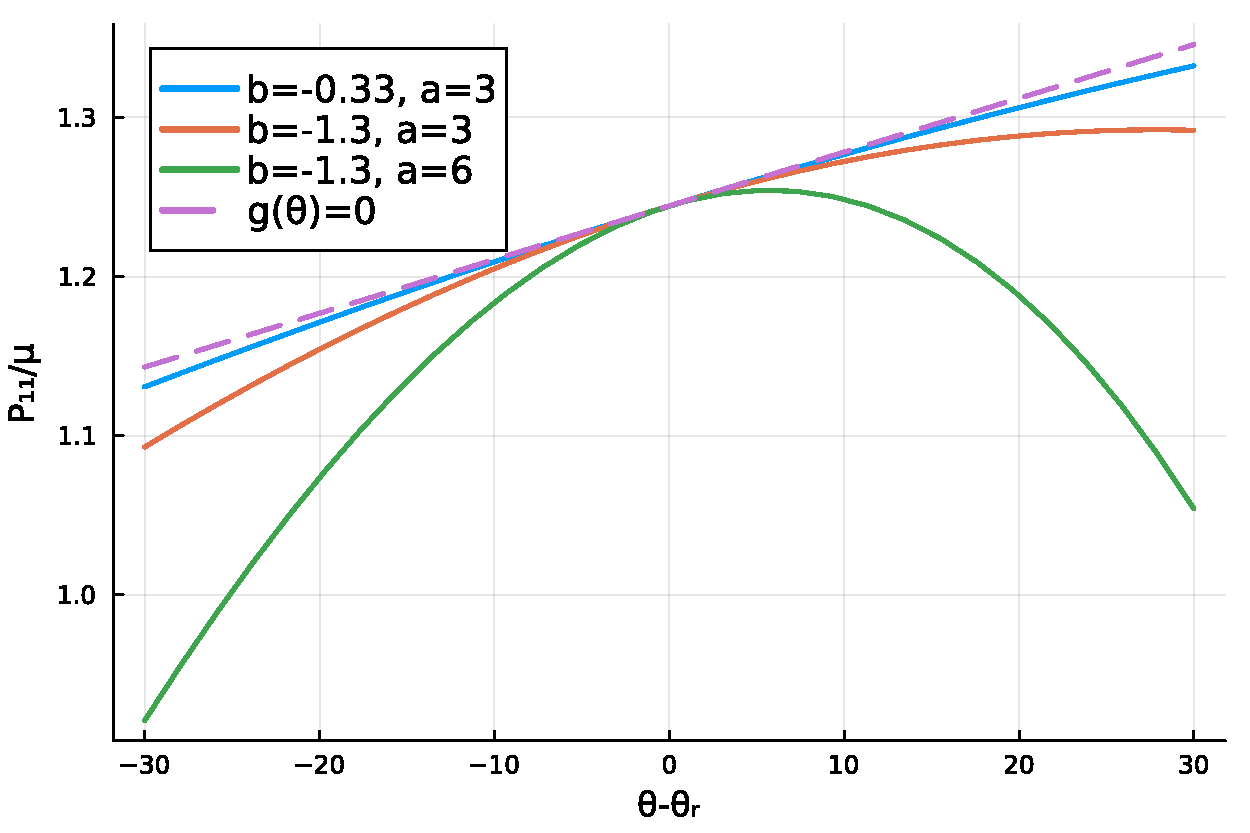
\includegraphics[width=0.45\textwidth]{Figures/NonlinearBehaviourTemperature}&
		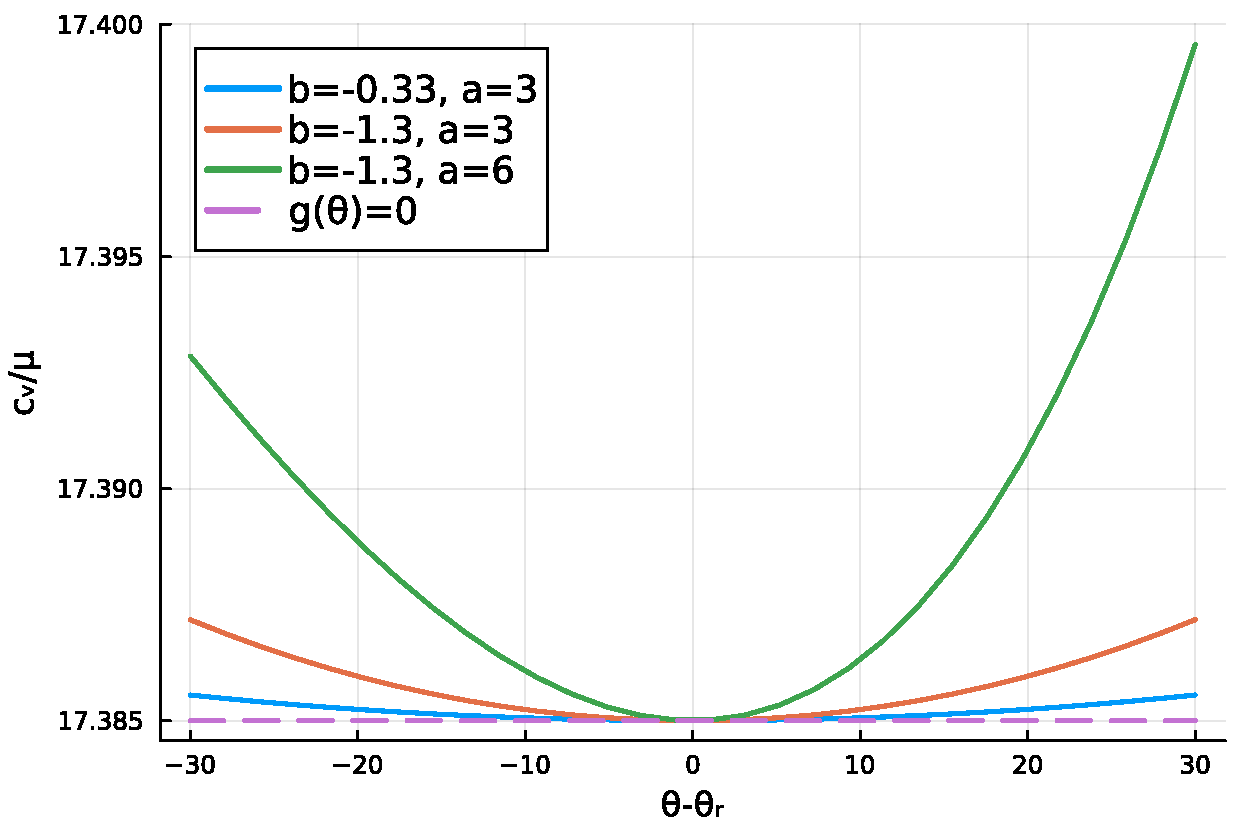
\includegraphics[width=0.45\textwidth]{Figures/Cv_vs_Temperature}\\
		%
		(a)  &  (b)
		%
	\end{tabular}
	\vspace{-2mm}
	\caption{a) Nonlinear behaviour of stress (component $11$ of $\vect{P}$) with respect to temperature; b) Nonlinear behaviour of $c_v$ with respect to $\theta$. In both cases  $\vect{F}$ and $\vect{E}_0$ have been fixed to the values given in \eqref{eqn:fixed values} where the purely mechanical and electro-mechanical isothermal potential,  $\Psi_m$ and $\Psi_{em}$ correspond with a Mooney-Rivlin model and  an ideal dielectric elastomer model, respectively.}
	\label{fig:model}
\end{figure}


\subsection{Specific forms of $\Psi_m(\vect{F})$ and $\Psi_{em}(\vect{F},\vect{E}_0)$}\label{sec:ground truth models}

In the generic expression of the Helmholtz energy density, $\Psi(\vect{F},\vect{E}_0,\theta)$, as presented in equation \eqref{eqn:additive decomposition}, we have systematically defined all terms except for $\Psi_{m}(\vect{F})$ and $\Psi_{em}(\vect{F},\vect{E}_0)$. For these two potentials, we have explored a broad spectrum of models that characterize the constitutive behavior of ideal dielectric elastomers under isothermal conditions. Specifically, for the purely mechanical contribution $\Psi_m(\vect{F})$, we have examined various hyperelastic potentials listed in Table \ref{table:mechanical potentials}, which include: 
 Mooney-Rivlin model; Quadratic Mooney-Rivlin model; Gent model;  Yeoh model; Arruda-Boyce model; Hyperelastic potentials for transverse isotropy. Table \ref{table:mechanical potentials}  presents the values of the material parameters employed in defining each of the aforementioned models. 

\begin{table}[htbp!]
	\centering
%	\arrayrulecolor{black} % Border color
%	\arrayrulewidth=1pt    % Border width
	\begin{tabular}{c c}
\rowcolor{gray!30}	\multicolumn{2}{c}{Mechanical isothermal Helmholtz free energy $\Psi_{m}$}		\\	
\midrule
\rowcolor{gray!30} {Name of the model}   &  Invariant representation		\\	
%
       \midrule % Border width
%
Mooney-Rivlin (MR) & $\mathbb{U}_{\Psi}  = \frac{\mu_1}{2} \left(I_{\Psi_1} - 3 \right) + \frac{\mu_2}{2} \left(I_{\Psi_2} - 3 \right) - \left( \mu_1 + 2\mu_2 \right) \text{ln} \left(I_{\Psi_3} \right) + \frac{\lambda}{2}  \left( I_{\Psi_3} - 1 \right)^2$\\
%
%    	\arrayrulecolor{black} % Border color
%	\begin{center}
\multicolumn{2}{c}{}\\
\multicolumn{2}{c}{\begin{tabular}{@{}lllll@{}}
		\toprule
		Parameter: & $\mu_1$  & $\mu_2$ & $\lambda$ & $\varepsilon$\\
		\midrule
		Value:    & $0.5$   & $0.5$  & $5$  & $1$\\
		\bottomrule
	\end{tabular}}\\

       \midrule % Border width

%
Quadratic MR (QMR)  &  $\mathbb{U}_{\Psi} = \frac{\mu_1}{2} \left(I_{\Psi_1} \right)^2 + \frac{\mu_2}{2} \left(I_{\Psi_2} \right)^2 - 6 \left( \mu_1 + 2\mu_2 \right) \text{ln} \left(I_{\Psi_3} \right) + \frac{\lambda}{2}  \left( I_{\Psi_3} - 1 \right)^2 $\\
%
%
\multicolumn{2}{c}{}\\

\multicolumn{2}{c}{\begin{tabular}{@{}lllll@{}}
		\toprule
		Parameter: & $\mu_1$  & $\mu_2$ & $\lambda$ & $\varepsilon$\\
		\midrule
		Value:    & $0.5$   & $0.5$  & $5$  &  $1$ \\
		\bottomrule
\end{tabular}}\\

%
%
       \midrule % Border width
       %
       %
       %
Gent (G)  &  $\mathbb{U}_{\Psi} = - \frac{\mu }{2}  J_m\text{ln}\left( 1 - \frac{I_{\Psi_1} - 3}{J_m} \right) - \mu \text{ln} \left(I_{\Psi_3} \right) + \frac{\lambda}{2}  \left( I_{\Psi_3} - 1 \right)^2 $\\
%
%
\multicolumn{2}{c}{}\\

\multicolumn{2}{c}{	\begin{tabular}{@{}lllll@{}}
		\toprule
		Parameter: & $\mu$  & $J_m$ & $\lambda$ & $\varepsilon$\\
		\midrule
		Value:    & $1$   & $19$ & $5$ & $1$ \\
		\bottomrule
\end{tabular}}\\
%
\midrule % Border width
Yeoh (Y) &  $\mathbb{U}_{\Psi} = C_{10} \left( I_{\Psi_1} - 3 \right) + C_{20} \left( I_{\Psi_1} - 3 \right)^2 + C_{30} \left( I_{\Psi_1} - 3 \right)^3 $\\&
$- 2 C_{10} \text{ln} \left(I_{\Psi_3} \right) + \frac{\lambda}{2}  \left( I_{\Psi_3} - 1 \right)^2  $\\
%
%
\multicolumn{2}{c}{}\\

\multicolumn{2}{c}{	\begin{tabular}{@{}llllll@{}}
		\toprule
		Parameter: & $C_{10}$  & $C_{20}$ & $C_{30}$ & $\lambda$ & $\varepsilon$\\
		\midrule
		Value:    & $1$   & $1$  & $1$ & $5$ & $1$  \\
		\bottomrule
	\end{tabular}}\\
%
\midrule % Border width
%
%
Arruda-Boyce (AB)  &  $\mathbb{U}_{\Psi} = a_1 \left( \beta \left(I_{\Psi_1} \right) \lambda_c \left(I_{\Psi_1} \right) - a_2 \text{ln} \left( \frac{\sinh \left( \beta \left(I_{\Psi_1} \right) \right)}{\beta \left(I_{\Psi_1} \right)} \right) \right)$\\&$ - A \text{ln} \left(I_{\Psi_3} \right) + \frac{\lambda}{2} \left( I_{\Psi_3} - 1 \right)^2  +B $\\
& $
\lambda_c \left(I_{\Psi_1} \right) = \sqrt{\frac{1}{3}}\sqrt{I_{\Psi_1}}; \qquad \mathcal{L}^{-1} \left( x \right) = \frac{3x - x^3}{1 - x^2}; \qquad \beta \left(I_1 \right) = \mathcal{L}^{-1} \left( \frac{\lambda_c \left(I_{\Psi_1} \right)}{a_2} \right) \nonumber
$\\
%
\multicolumn{2}{c}{}\\

\multicolumn{2}{c}{	\begin{tabular}{@{}lllll@{}}
		\toprule
		Parameter: & $a_1$  & $a_2$ & $\lambda$ & $\varepsilon$\\
		\midrule
		Value:    & $2.1899$   & $\sqrt{6}$ & $4.9159$  &  $1$ \\
		\bottomrule
\end{tabular}}\\
%
\midrule % Border width
 %
 %
Trans. Isotropy (TI)  &$
\mathbb{U}_{\Psi} = \frac{\mu_1}{2} \left(I_{\Psi_1} - 3 \right) + \frac{\mu_2}{2} \left(I_{\Psi_2} - 3 \right) - \left( \mu_1 + 2\mu_2 + \mu_3 \right) \text{ln} \left(I_{\Psi_3} \right)$ \\&
$+ \frac{\lambda}{2}  \left( I_{\Psi_3} - 1 \right)^2	+ \frac{\mu_3}{2 \alpha} \Big(\left(I_{\Psi_6} \right)^{\alpha}-1\Big) + \frac{\mu_3}{2 \beta}\Big( \left(I_{\Psi_7} \right)^{\beta} -1\Big)$	 
\\
%
\multicolumn{2}{c}{}\\

\multicolumn{2}{c}{	\begin{tabular}{@{}lllllllll@{}}
		\toprule
		Parameter: & $\mu_1$  & $\mu_2$ & $\mu_3$ & $\lambda$ & $\alpha$ & $\beta$ & $\varepsilon$ & $\bm{N}$ \\
		\midrule
		Value:    & $0.5$   & $0.5$  & $7.5$ & $5$ & $2$ & $2$ & $1$ & $\frac{1}{\sqrt{3}}\begin{bmatrix}1& 1& 1 \end{bmatrix}^T$ \\
		\bottomrule
\end{tabular}}\\
%
\midrule % Border width
       
       
%\end{center}
	\end{tabular}
%
	\caption{The various models used for the isothermal mechanical contribution $\Psi_{m}(\vect{F})$ in \eqref{eqn:additive decomposition}.}
	\label{table:mechanical potentials}
\end{table}


With regards to the electro-mechanical contribution $\Psi_{em}(\vect{F},\vect{E}_0)$, we have considered: Ideal dielectric elastomer; Model with electric saturation, employed by some authors to account for the saturation effects associated with hard inclusions that exhibit electric saturation. Both models and the material parameters used in their definition can be seen in Table \ref{table: electromechanical models}.


\begin{table}[htbp!]
	\centering
	%	\arrayrulecolor{black} % Border color
	%	\arrayrulewidth=1pt    % Border width
	\begin{tabular}{c c}
		\rowcolor{gray!30}	\multicolumn{2}{c}{Electro-mechanical isothermal Helmholtz free energy $\Psi_{em}$}		\\	
		\midrule
		\rowcolor{gray!30} {Name of the model}   &  Invariant representation		\\	
		%
		\midrule % Border width
		%
		Ideal dielectric (ID) & $\mathbb{U}_{\Psi}  = \frac{\mu_1}{2} \left(I_{\Psi_1} - 3 \right) + \frac{\mu_2}{2} \left(I_{\Psi_2} - 3 \right) - \left( \mu_1 + 2\mu_2 \right) \text{ln} \left(I_{\Psi_3} \right) + \frac{\lambda}{2}  \left( I_{\Psi_3} - 1 \right)^2$\\
		%
		%    	\arrayrulecolor{black} % Border color
		%	\begin{center}
		\multicolumn{2}{c}{}\\
		\multicolumn{2}{c}{\begin{tabular}{@{}lllll@{}}
				\toprule
				Parameter: & $\mu_1$  & $\mu_2$ & $\lambda$ & $\varepsilon$\\
				\midrule
				Value:    & $0.5$   & $0.5$  & $5$  & $1$\\
				\bottomrule
		\end{tabular}}\\
		
		\midrule % Border width
		
		%
		Electric Saturation (ES)  &  $\mathbb{U}_{\Psi} = \frac{\mu_1}{2} \left(I_{\Psi_1} \right)^2 + \frac{\mu_2}{2} \left(I_{\Psi_2} \right)^2 - 6 \left( \mu_1 + 2\mu_2 \right) \text{ln} \left(I_{\Psi_3} \right) + \frac{\lambda}{2}  \left( I_{\Psi_3} - 1 \right)^2 $\\
		%
		%
		\multicolumn{2}{c}{}\\
		
		\multicolumn{2}{c}{\begin{tabular}{@{}lllll@{}}
				\toprule
				Parameter: & $\mu_1$  & $\mu_2$ & $\lambda$ & $\varepsilon$\\
				\midrule
				Value:    & $0.5$   & $0.5$  & $5$  &  $1$ \\
				\bottomrule
		\end{tabular}}\\
		
		%
		%
	
		\midrule % Border width
		
		
		%\end{center}
	\end{tabular}
	%
	\caption{The two models used for the isothermal electro-mechanical contribution $\Psi_{em}(\vect{F},\vect{E}_0)$ in \eqref{eqn:additive decomposition}.}
	\label{table: electromechanical models}
\end{table}





\newpage
%



\section{Physics-augmented neural networks constitutive models}\label{eqn:calibration strategies}

In the preceding section, we introduced the general form of the analytical Helmholtz free energy density, which serves as the foundation for generating in-silico data in this section. The primary goal here is to generate such data with Helmholtz free energy densities that are decomposed as per equation \eqref{eqn:additive decomposition}, depending on ${\vect{F},\vect{E}_0,\theta}$. This approach aims to facilitate the construction of neural network surrogates with the capability to depend on the sets $\{\vect{F},\vect{E}_0,\theta\}$, $\{\vect{F},\vect{D}_0,\eta\}$, $\{\vect{F},\vect{D}_0,\theta\}$, or $\{\vect{F},\vect{E}_0,\eta\}$, as outlined in Section \ref{sec:alternative potentials}. These surrogates are consistently denoted as $\Psi_{nn}$, $e_{nn}$, $\Upsilon_{nn}$, or $\Gamma_{nn}$, respectively, in alignment with the potentials described in Section \ref{sec:alternative potentials}.

Crucially, to ensure compliance with fundamental physical principles, such as material frame indifference and material symmetry, we follow an invariant formulation for these potentials, as detailed in Section \ref{subsec:InvariantFormulation}. All of this  is mathematically encapsulated in equation \eqref{eqn:NN objective}, i.e
%
\begin{equation}\label{eqn:NN objective}
\boxed{\begin{aligned}	
&\begin{aligned}
&\text{Ground truth model}\\
&\text{in equation \eqref{eqn:additive decomposition}}
\end{aligned}&
\begin{aligned}
&\text{Family of data-driven neural network}\\
&\text{thermodynamical potentials}
\end{aligned}\\
\hline\\
%
&\Psi(\vect{F},\vect{E}_0,\theta) &\left\{\begin{aligned}
\Psi_{nn}(\vect{F},\vect{E}_0,\theta,\vect{\mathcal{W}})&=\mathbb{U}_{\Psi\,nn}\left(I_{\Psi_1},\dots,I_{\Psi_{n_{\text{inv}}}},\theta\right)\\
e_{nn}(\vect{F},\vect{D}_0,\eta,\vect{\mathcal{W}})&=\mathbb{U}_{e\,nn}\left(I_{e_1},\dots,I_{e_{n_{\text{inv}}}},\eta\right)\\
\Upsilon_{nn}(\vect{F},\vect{D}_0,\theta,\vect{\mathcal{W}})&=\mathbb{U}_{\Upsilon\,nn}\left(I_{\Upsilon_1},\dots,I_{\Upsilon_{n_{\text{inv}}}},\theta\right)\\
\Gamma_{nn}(\vect{F},\vect{E}_0,\eta,\vect{\mathcal{W}})&=\mathbb{U}_{\Gamma\,nn}\left(I_{\Gamma_1},\dots,I_{\Gamma_{n_{\text{inv}}}},\eta\right)
\end{aligned}\right.\\
%
%
\end{aligned}}
\end{equation}
%

In equation \eqref{eqn:NN objective}, $\vect{\mathcal{W}}$ represents the parameters of the neural network, which encompass
%
\begin{equation}
\vect{\mathcal{W}}=\left\{\vect{W}_1,\dots,\vect{W}_{n_{L+1}},\vect{b}_1,\dots,\vect{b}_{n_{L+1}}\right\},
\end{equation}
%
where $\vect{W}_i$ and $\vect{b}_i$ represent the weights and biases associated with layer $i$. As standard in neural networks, for an architecture with $n_{L+1}$ layers, the inputs $\vect{A}_h$ of layer $h$ is obtained through the following expression
%
\begin{equation}
\vect{A}_h   =  \sigma_h\left(\vect{W}_h\vect{A}_{h-1}+\vect{b}_h\right);\qquad h=\{1,\dots,n_{L+1}\}
\end{equation}
%
where 
%
\begin{equation}
\begin{aligned}
\vect{W}_h  \in \mathbb{R}^{n_{h}\times n_{h-1}};\qquad 	\vect{b}_h  \in \mathbb{R}^{n_{h}}
\end{aligned}
\end{equation}
%
where
%
\begin{equation}
n_0  =  n_{\text{inv}}+1;\qquad n_{L+1}=1
\end{equation}
%
where $n_{\text{inv}}=5$ or $n_{\text{inv}}=8$ for isotropy or transverse isotropy, respectively. Furthermore, the vectors $\vect{A}_h$, for $h=L+1$ represents the predicted neural network model whereas for $h=0$, it represents the input of the model, namely 
%
\begin{equation}
\begin{aligned}
\vect{A}_{L+1}&  =  \Psi_{nn}(\vect{F},\vect{E}_0, \theta,\vect{\mathcal{W}});&\qquad \vect{A}_0&  =  \begin{bmatrix}
I_{\Psi_1}  &  I_{\Psi_2} & \dots & I_{\Psi_n} & \theta
\end{bmatrix}\\
%
\vect{A}_{L+1}&  =  e_{nn}(\vect{F},\vect{D}_0, \eta,\vect{\mathcal{W}});&\qquad \vect{A}_0 & =  \begin{bmatrix}
I_{e_1}  &  I_{e_2} & \dots & I_{e_n} & \eta
\end{bmatrix}\\
%
\vect{A}_{L+1}&  = \Upsilon_{nn}(\vect{F},\vect{D}_0, \theta,\vect{\mathcal{W}});&\qquad\vect{A}_0 & =  \begin{bmatrix}I_{\Upsilon_1}  &  I_{\Upsilon_2} & \dots & I_{\Upsilon_n} & \theta
\end{bmatrix}\\
%
\vect{A}_{L+1}&  = \Gamma_{nn}(\vect{F},\vect{E}_0, \eta,\vect{\mathcal{W}});&\qquad\vect{A}_0 & =  \begin{bmatrix}I_{\Gamma_1}  &  I_{\Gamma_2} & \dots & I_{\Gamma_n} & \eta
\end{bmatrix}
\end{aligned}
\end{equation}

In addition, $\sigma_h$ represents the activation function of laer $h$. In our work we have made use of Softplus activation functions, except for the last layer, where we use the identity function, namely
%
\begin{equation}\label{eqn:activation functions}
\sigma_h(x)=\log\left(1 + e^x\right),\,\,h=\{1,\dots,n_L\};\qquad \sigma_{n_{L+1}}(x)=x
\end{equation}

\subsection{Sobolev-type calibration strategy 1}\label{sec:strategy 1}
 
 We begin by describing the fundamental aspects of this strategy (Section \ref{sec:fundamentals strategy 1}), and later, we describe the in-silico data generation strategy used in order to calibrated the models according to this strategy, carried out in Section \ref{sec:data generation strategy 1}.

\subsubsection{Fundamental aspects of the strategy}\label{sec:fundamentals strategy 1}

In this approach, four distinct types of neural network models, namely $\Psi_{nn}(\vect{F},\vect{E}_0,\theta,\vect{\mathcal{W}})$, $e_{nn}(\vect{F},\vect{D}_0,\eta,\vect{\mathcal{W}})$, 
$\Upsilon_{nn}(\vect{F},\vect{D}_0,\theta,\vect{\mathcal{W}})$ or
$\Gamma_{nn}(\vect{F},\vect{E}_0,\eta,\vect{\mathcal{W}})$, are developed with the specific objective of minimizing the discrepancy between: 
%
\begin{itemize}
	\item  the derivatives  $\{\partial_{\vect{F}}\Psi_{nn},-\partial_{\vect{E}_0}\Psi_{nn},-\partial_{\theta}\Psi_{nn}\}$ and $\{\vect{P},\vect{D}_0,\eta\}:=\{\partial_{\vect{F}}\Psi,-\partial_{\vect{E}_0}\Psi,-\partial_{\theta}\Psi\}$
	%
	\item  the derivatives  $\{\partial_{\vect{F}}e_{nn},\partial_{\vect{D}_0}e_{nn},\partial_{\eta}e_{nn}\}$ and $\{\vect{P},\vect{E}_0,\theta\}:=\{\partial_{\vect{F}}\Psi,{\vect{E}_0},\theta\}$
	%
	\item  the derivatives  $\{\partial_{\vect{F}}\Upsilon_{nn},\partial_{\vect{D}_0}\Upsilon_{nn},-\partial_{\theta}\Upsilon_{nn}\}$ and $\{\vect{P},\vect{E}_0,\eta\}:=\{\partial_{\vect{F}}\Psi,{\vect{E}_0},-\partial_{\eta}\Psi\}$	
	%
	\item  the derivatives  $\{\partial_{\vect{F}}\Gamma_{nn},-\partial_{\vect{E}_0}\Gamma_{nn},\partial_{\eta}\Gamma_{nn}\}$ and $\{\vect{P},\vect{D}_0,\theta\}:=\{\partial_{\vect{F}}\Psi,-\partial_{\vect{E}_0}\Psi,\theta\}$	
\end{itemize}
%
showcasing that, regardless of the neural network surrogate employed, the underlying ground truth model remains a Helmholtz free energy density $\Psi(\vect{F},\vect{E}_0,\theta)$ as formulated in equation \eqref{eqn:additive decomposition}. This is illustrated schematically in Figure \ref{fig:strategy 1}.
To accomplish this objective, we define the corresponding Sobolev-type loss functions, with their specific expressions provided in Table \ref{table: sobolev type 1}.

\begin{table}[htbp!]
	\centering
	\begin{tabular}{c c c}
		\toprule
		\rowcolor{gray!30}	\small{} & $\mathcal{L}(\vect{\mathcal{W}})$ &\\
		\midrule
 $\Psi_{nn}$	&	\begin{minipage}{0.72\textwidth}
			\begin{equation*}
			\begin{aligned}
			& \beta_1\frac{\sum_{i=1}^{n_{\text{d}}} \left\| \partial_{\vect{F}}\Psi^{i} - \partial_{\vect{F}} \Psi_{nn}(\vect{X}^i, \vect{\mathcal{W}}) \right\|^2}{\sum_{i=1}^{n_{\text{d}}} \left\| \partial_{\vect{F}}\Psi^{i} \right\|^2}  + \beta_2\frac{\sum_{i=1}^{n_{\text{d}}} \left\| \partial_{\vect{E}_0}\Psi^{i} - \partial_{\vect{E}_0} \Psi_{nn}(\vect{X}^i, \vect{\mathcal{W}}) \right\|^2}{\sum_{i=1}^{n_{\text{d}}} \left\| \partial_{\vect{E}_0}\Psi^{i} \right\|^2} \\
			& + \beta_3\frac{\sum_{i=1}^{n_{\text{d}}} \Big( \partial_{\theta}\Psi^{i} - \partial_{\theta} \Psi_{nn}(\vect{X}^i, \vect{\mathcal{W}}) \Big)^2}{\sum_{i=1}^{n_{\text{d}}} \left( \partial_{\theta}\Psi^{i} \right)^2}
			\end{aligned}
			\end{equation*}
		\end{minipage}  & $\vect{X}^i=\{\vect{F}^i, \vect{E}_0^i, \theta^i\}$ \\
		%	
		\midrule
		%
 $e_{nn}$	&	\begin{minipage}{0.72\textwidth}
			\begin{equation*}
			\begin{aligned}
			& \beta_1\frac{\sum_{i=1}^{n_{\text{d}}} \left\| \partial_{\vect{F}}\Psi^{i} - \partial_{\vect{F}} e_{nn}(\vect{X}^i, \vect{\mathcal{W}}) \right\|^2}{\sum_{i=1}^{n_{\text{d}}} \left\| \partial_{\vect{F}}\Psi^{i} \right\|^2}  + \beta_2\frac{\sum_{i=1}^{n_{\text{d}}} \left\| \vect{E}_0^{i} - \partial_{\vect{D}_0} e_{nn}(\vect{X}^i, \vect{\mathcal{W}}) \right\|^2}{\sum_{i=1}^{n_{\text{d}}} \left\| \vect{E}_0^{i} \right\|^2} \\
			& + \beta_3\frac{\sum_{i=1}^{n_{\text{d}}} \left( \theta^{i} - \partial_{\eta} e_{nn}(\vect{X}^i, \vect{\mathcal{W}}) \right)^2}{\sum_{i=1}^{n_{\text{d}}} \left( \theta^{i} \right)}
			\end{aligned}
			\end{equation*}
		\end{minipage}  & $\vect{X}^i=\{\vect{F}^i, -\partial_{\vect{E}_0}\Psi^i, -\partial_{\theta}\Psi^i\}$ 	\\
		%
		\midrule
		%
 $\Upsilon_{nn}$ &		\begin{minipage}{0.68\textwidth}
			\begin{equation*}
			\begin{aligned}
			& \frac{\sum_{i=1}^{n_{\text{d}}} \left\| \partial_{\vect{F}}\Psi^{i} - \partial_{\vect{F}} \Upsilon_{nn}(\vect{X}^i, \vect{\mathcal{W}}) \right\|^2}{\sum_{i=1}^{n_{\text{d}}} \left\| \partial_{\vect{F}}\Psi^{i} \right\|^2}  + \frac{\sum_{i=1}^{n_{\text{d}}} \left\| \vect{E}_0^{i} - \partial_{\vect{D}_0} \Upsilon_{nn}(\vect{X}^i, \vect{\mathcal{W}}) \right\|^2}{\sum_{i=1}^{n_{\text{d}}} \left\| \vect{E}_0^{i} \right\|^2} \\
			& + \frac{\sum_{i=1}^{n_{\text{d}}} \left( \partial_{\theta}\Psi^{i} - \partial_{\theta} \Upsilon_{nn}(\vect{X}^i, \vect{\mathcal{W}}) \right)^2}{\sum_{i=1}^{n_{\text{d}}} \left( \partial_{\theta}\Psi^{i} \right)^2}
			\end{aligned}
			\end{equation*}
		\end{minipage}  & $\vect{X}^i=\{\vect{F}^i, -\partial_{\vect{E}_0}\Psi^i, \theta^i\}$ 	\\
		%
		\midrule
		%
 $\Gamma_{nn}$	&	\begin{minipage}{0.68\textwidth}
			\begin{equation*}
			\begin{aligned}
			& \frac{\sum_{i=1}^{n_{\text{d}}} \left\| \partial_{\vect{F}}\Psi^{i} - \partial_{\vect{F}} \Gamma_{nn}(\vect{X}^i, \vect{\mathcal{W}}) \right\|^2}{\sum_{i=1}^{n_{\text{d}}} \left\|\partial_{\vect{F}}\Psi^{i} \right\|^2}  + \frac{\sum_{i=1}^{n_{\text{d}}} \left\| \partial_{\vect{E}_0}\Psi^{i} - \partial_{\vect{E}_0} \Gamma_{nn}(\vect{X}^i, \vect{\mathcal{W}}) \right\|^2}{\sum_{i=1}^{n_{\text{d}}} \left\| \partial_{\vect{E}_0}\Psi^{i} \right\|^2} \\
			& + \frac{\sum_{i=1}^{n_{\text{d}}} \left( \theta^{i} - \partial_{\eta} \Gamma_{nn}(\vect{X}^i, \vect{\mathcal{W}}) \right)^2}{\sum_{i=1}^{n_{\text{d}}} \left( \theta^{i} \right)^2}
			\end{aligned}
			\end{equation*}
		\end{minipage} & $\vect{X}^i=\{\vect{F}^i, \vect{E}_0^i, -\partial_{\theta}\Psi^i\}$	\\
		\midrule
		
		
		%
	\end{tabular}
	\caption{Loss functions $\mathcal{L}(\vect{\mathcal{W}})$ used for the calibration of the various type of neural network-based surrogate potentials, i.e. $\Psi_{nn}$, $e_{nn}$, $\Upsilon_{nn}$ or $\Gamma_{nn}$, for the case of Sobolev-type training strategy 1. All the potentials have been calibrated with data obtained from Helmholtz free energy density ground truth models, i.e. $\Psi$. The index $i$ represents in-silico data number $i$, and $n_d$ the number of data used for calibration.}
	\label{table: sobolev type 1}
\end{table}






\begin{figure}[htpb!]
	\centering
	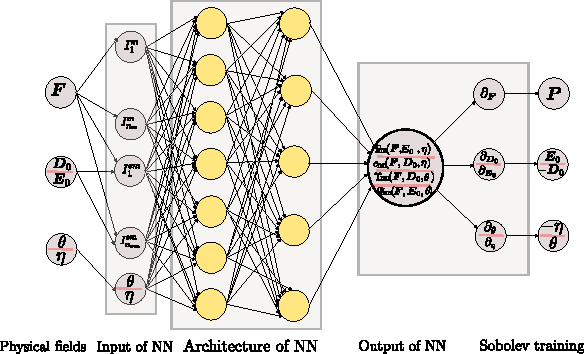
\includegraphics[width=0.85\textwidth]{Figures/InkScape/NN_1}\\
	\vspace{-2mm}
	\caption{Simplified structure of the neural network architecture used for calibration of the four neural network-based surrogate potentials i.e. $\Psi_{nn}$, $e_{nn}$, $\Upsilon_{nn}$ or $\Gamma_{nn}$, for the case of Sobolev-type training strategy 1.}
	\label{fig:strategy 1}
\end{figure}


\subsubsection{Polyconvexity of neural network-based potentials}

Sections \ref{sec:helmholtz} and \ref{sec:alternative potentials} described the desired convexity/convexity conditions that the four possible neural network-based thermodycanimical potentials, namely $\Psi(\vect{F},\vect{E}_0,\theta)$, $e\vect{F},\vect{D}_0,\eta)$, $\Upsilon(\vect{F},\vect{D}_0,\theta)$ or $\Gamma(\vect{F},\vect{E}_0,\theta)$ should satisfy. 
Enforcing simultaneous convexity and convexity across multiple physics, as required for the three potentials $\Psi(\vect{F},\vect{E}_0,\theta)$,  $\Upsilon(\vect{F},\vect{D}_0,\theta)$ or $\Gamma(\vect{F},\vect{E}_0,\theta)$, presents a complex challenge. This difficulty arises whether the model is derived from a phenomenological explicit representation or constructuted using neural network frameworks. However, the direct imposition of convexity exclusively, or more specifically, polyconvexity in the sense of equation \eqref{eqn:polyconvexity}, proves to be more tractable. Building on the work of XX and extending it from electro-mechanics to the thermo-electro-mechanical context, a sufficient condition to ensure polyconvexity of the neural network-based potential $e_{nn}(\vect{F},\vect{D}_0,\eta)$ is the positiveness of the weights $\vect{W}_{h}$ and the monotonically increasing nature of the activation functions, namely
%
\begin{equation}
	\left(\vect{W}_h\right)_{ij}>0;\qquad \sigma^{\prime}_h(x)>0,\forall x;\qquad  h=\left\{1,\dots,n_{L+1}\right\}
\end{equation}

Notice that the first condition can be imposed as a penalty term in the objective function, leading to the augmented objective function $\widetilde{\mathcal{L}}(\vect{\mathcal{W}})$ defined as
%
\begin{equation}
	\widetilde{\mathcal{L}}(\vect{\mathcal{W}})=\mathcal{L}(\vect{\mathcal{W}}) + \frac{\kappa}{2} \sum_{i}\Big(\min\left(\left(\vect{\mathcal{W}}_v\right)_i,0\right)\Big)^2
\end{equation}
%
where $\mathcal{L}(\vect{\mathcal{W}})$ is defined as in Table \ref{table: sobolev type 1}, $\vect{\mathcal{W}}_v$ represents the concatenation of all vectorized weights $\vect{\mathcal{W}}_h$, $h=\{1,\dots,n_{L+1}\}$, and $\kappa$, the penalty parameter. Furthermore, notice that increasing monotonicity is satisfied by the activation functions chosen in equation \eqref{eqn:activation functions}. In this work, we will explore the accuracy of neural network-based $e_{nn}(\vect{F},\vect{D}_0,\eta)$ potentials with and without the additional penalty term enforcing the polyconvexity condition. This will be futher discussed in Section \ref{sec:polyconvexity}.





\subsubsection{In-silico data generation strategy}\label{sec:data generation strategy 1}

In this section, we present the procedure used for generating synthetic data for the training strategy denoted as strategy 1. For that, we have made use of the generic form of the Helmholtz free energy density in equation \eqref{eqn:additive decomposition}, and a variety of models for the isothermal purely mechanical and electro-mechanical contributions $\Psi_m(\vect{F}$ (see Table \ref{table:mechanical potentials}) and $\Psi_{em}(\vect{F},\vect{E}_0)$ (refer to Table \ref{table: electromechanical models}).

To acquire the dataset, we have adhered to the procedure outlined in \cite{OKunc_19_01}, extended to the coupled context of thermo-electro-mechanics. The deformation gradient tensor $\vect{F}$ is parameterized via a  chosen set of deviatoric directions, amplitudes, and Jacobians ($J$, i.e., the determinant of $\vect{F}$). The process of generating sample points for deviatoric directions, amplitudes, and Jacobians is elucidated in Algorithm \ref{alg:sample_generation}. Similarly, the electric displacement $\vect{E}_0$ (for the neural network-based potentials $\Psi_{nn}(\vect{F},\vect{E}_0,\theta)$ and $\Upsilon_{nn}(\vect{F},\vect{E}_0,\eta)$) or $\vect{D}_0$ (for the neural network-based potentials $e_{nn}(\vect{F},\vect{D}_0,\eta)$ and $\Gamma_{nn}(\vect{F},\vect{D}_0,\theta)$) is also parametrised in terms of unitary directions and amplitudes.
Concerning the deviatoric directions for $\vect{F}$, denoted as $\vect{V_F}$ we formulate them using a spherical parametrization in $\mathbb{R}^5$, precisely representing these directions using five pertinent angular measures ($\phi_1, \phi_2, \phi_3, \phi_4, \phi_5\in[0,2\pi]\times[0,\pi]\times[0,\pi]\times[0,\pi]\times[0,\pi]$) within this 5-dimensional space.  For the directions employed for the parametrisation of $\vect{E}_0$  or $\vect{D}_0$ (depending on the dependence on the electrical physics of the neural network-based potential), denoted as $\vect{V}_{\vect{E}_0}$ or $\vect{V}_{\vect{D}_0}$, respectively, these are created using a spherical parametrization in $\mathbb{R}^3$, using as angular measures $(\theta,\psi)\in[0,2\pi]\times[0,\pi]$, namely
%
%

\begin{algorithm}
	\caption{Pseudo-code for sample generation}
	\label{alg:sample_generation}
	
	\begin{algorithmic}[1]
		\State Generate deformation gradient tensors $\vect{F}$ according to:
		
		\begin{algorithmic}[1]
			\State Set the number of amplitudes, directions and determinants: $\{ n_{\bm{t}_{\vect{F}}}, n_{\bm{V}_{\vect{F}}}, n_{\bm{J}_{\vect{F}}}\}$;
			
			\State Initialise a vector of Latin Hypercube Sampled angles: $\bm{\phi}_1 = [0,2\pi]_{n_{\bm{V_F}} \times 1}$ and  $\bm{\phi}_{2,...,4} = [0,\pi]_{n_{\bm{V_F}} \times 1}$;
			
			\State Construct the directions, $\bm{V}_{F}$, using $\bm{\phi}_1, \dots, \bm{\phi}_4$ by means of an extended Spherical parametrisation in $\mathbb{R}^5$ - detailed in (\ref{eqn:spherical_parametersisation});
			
			\State Evaluate the deformation gradient tensors, $\bm{{F}}$ - detailed in Algorithm \ref{alg:F_construction};
		\end{algorithmic}
		
		\State{Generate electric field vectors $\vect{E}_0$ (or $\vect{D}_0$) according to:}
		
		\begin{algorithmic}[1]
			\State Set the amplitudes and directions: $\{n_{\bm{t}_{\vect{E}_0}},  n_{\bm{V}_{\vect{E}_0}}\}$;
			
			\State Initialise a vector of Latin Hypercube Sampled angles: $\bm{\psi}_1 = [0,2\pi]_{n_{\bm{V}_{\vect{E}_0}} \times 1}$ and  $\bm{\psi}_{2} = [0,\pi]_{n_{\bm{V}{\vect{E}_0}} \times 1}$;
			
			\State Construct the directions, $\bm{V}_{\bm{E}_0}$ (or $\vect{V}_{\vect{D}_0}$), using $\bm{\psi}_1, \bm{\psi}_2$ by means of a Spherical parametrisation in $\mathbb{R}^3$;
			
			\State Evaluate the deformation $\bm{{E}}_0$ (or $\bm{{D}}_0$) - detailed in Algorithm \ref{alg:F_construction};
		\end{algorithmic}
		
		\State Generate temperature data $\theta$ (or entropy $\eta$) according to:
		
		\begin{algorithmic}[1]
			\State Set the maximum temperature difference with respect to $\theta_R$, denoted $\Delta\theta$. Then define the minimum and maximum values of $\theta$: $\theta_R-\Delta\theta$ and $\theta_R+\Delta\theta$; For $\eta$-based potentials, set $\eta_{\text{min}}$ and $\eta_{\text{max}}$
			
			\State Set number of temperatures $n_{\theta}$ (or $n_{\eta}$);
			
			\State Generate $n_{\theta}$ uniformly distributed temperature (or randomly) in the interval $(\theta_R-\Delta\theta,\theta_R+\Delta\theta)$; For $\eta$-based potentials, the interval is $(\eta_{\text{min}},\eta_{\text{max}})$
		\end{algorithmic}
		
		\State Generate combination of data of $\{\vect{F},\vect{E}_0,\theta\}$ (or any other combination, for instance $\{\vect{F},\vect{D}_0,\eta\}$)
	\end{algorithmic}
	
\end{algorithm}


%\input{section/05_Numerical_Examples/numerical_examples_sample_gen_algorithm}


%
\begin{equation}
\label{eqn:spherical_parametersisation}
\bm{V}_{\vect{F}}^i = 
\begin{bmatrix}
\cos{\phi_1^i} \\
\sin{\phi_1^i}\cos{\phi_2^i} \\
\sin{\phi_1^i}\sin{\phi_2^i}\cos{\phi_3^i} \\
\sin{\phi_1^i}\sin{\phi_2^i}\sin{\phi_3^i}\cos{\phi_4^i} \\
\sin{\phi_1^i}\sin{\phi_2^i}\sin{\phi_3^i}\sin{\phi_4^i}
\end{bmatrix};\,\, 1\leq i\leq n_{\bm{V_F}};\qquad 
%	
\bm{V}_{\vect{E}_0}^i=\begin{bmatrix}
\cos\psi_1^i\sin\psi_2^i\\  \sin\psi_1^i\sin\psi_2^i\\  \cos\psi_2^i\end{bmatrix};\,\, 1\leq i\leq n_{\bm{V}_{\vect{E}_0}}
\end{equation} 




Once the sample is generated following Algorithm \ref{alg:sample_generation}, the reconstruction of the deformation gradient tensor $\vect{F}$ and of $\vect{D}_0$ becomes possible at each of the sampling points. This reconstruction process is demonstrated in Algorithm \ref{alg:F_construction}, where $\bm{\Uppsi}$ represents the basis for symmetric and traceless tensors (refer to Appendix \ref{sec:appendix_basis_symm_traceless_tensors} for details on $\bm{\Uppsi}$). For the temperature field $\theta$, data generation has been carried out by predefining the maximum difference with respect to the reference temperature $\theta_R$. This approach establishes the lower and upper bounds $\theta_R-\Delta\theta$ and $\theta_R+\Delta\theta$.  Consequently, the data for this field is generated either uniformly distributed within this interval or randomly sampled across the defined range.




\begin{algorithm}[htbp!]
	\caption{Pseudo-code for construction of the set of deformation gradient tensors and electric  fields $\vect{E}_0$ (similarly for $\vect{D}_0$)}
	\label{alg:F_construction}  
	\begin{algorithmic}[1]                                                     
		\For{$i = 1:n_{\bm{V_F}}$}
		
		\For{$j = 1:n_J$}
		
		\For{$k = 1:n_{\bm{t_F}}$}
		
		\State $\bm{F} = J_j^{1/3} \exp\left([\vect{t}_{\vect{F}}]_k \left[\sum_{m = 1}^{5} [\vect{V}^i_{\vect{F}}]_m \bm{\Uppsi}_{m}\right] \right)$;	            		
		\EndFor
		\EndFor
		\EndFor
		
		\For{$i = 1:n_{\bm{V}_{\vect{E}_0}}$}		
		\For{$j = 1:n_{\bm{t}_{\vect{E}_0}}$}
\State $\bm{E}_0 = [\vect{t}_{\vect{E}_0}]_j\vect{V}^i_{\vect{E}_0}$;
\EndFor
\EndFor
		
		
		
	\end{algorithmic}
\end{algorithm}                         



\newpage

\subsection{Sobolev-type calibration strategy 2}\label{sec:strategy 2}

The calibration approach outlined in Section \ref{sec:strategy 1}, referred to as calibration strategy 1, is characterized by its remarkable flexibility—enabling the calibration of four distinct types of thermodynamic potentials—and its robustness, as demonstrated in the numerical examples section. However, this approach is subject to criticism when applied to scenarios involving data generated in real-world conditions, as opposed to an in-silico process. While calibration strategy 1 is well-suited for data generated in-silico, as is the case in this study, its applicability may be severely limited when dealing with laboratory-derived data. The primary challenge arises from the requirement for data across six quantities: $\{\vect{F},\vect{E}_0,\theta,\vect{P},\vect{D}_0,\eta\}$. Of these, entropy $(\eta)$ cannot be directly measured in a laboratory setting, which significantly impairs the feasibility of this calibration strategy in practical, real-world scenarios.


To address this limitation, we have developed an alternative strategy that can be applied to both in-silico and experimentally generated data. The key aspect of this approach lies in substituting the only non-measurable field within $\{\vect{F},\vect{E}_0,\theta,\vect{P},\vect{D}_0,\eta\}$, namely $\eta$, with other thermophysical properties that can be directly measured in a laboratory setting. This modification enhances the versatility of the calibration process, making it applicable to real-world experimental data as well as computationally generated scenarios. A suitable physical property to replace $\eta$ is the specific heat capacity $c_v$ (see equation \eqref{eqn:heat capacity}). 

As discussed in Section \ref{sec:ground truth model},  specifically for the generic Helmholtz free energy density considered in this study, $c_v$ may exhibit a nonlinear dependence on the fields fields $\{\vect{F},\vect{E}_0,\theta\}$, as highlighted in the experimental work of XX. Therefore, we consider incorporating data values for $c_v$ at a set of points $\mathcal{G}_{c_v}=\{\vect{X}^1,\dots,\vect{X}^{n_{c_v}}\}$, which includes the reference configuration $\vect{X}^1=\{\vect{I},\vect{0},\theta_R\}$ as well as other possible scenarios
$\vect{X}^i=\{\vect{F}^i,\vect{E}_0^i,\theta^i\}$, with $n_{c_v}$ the number of data points within the set $\mathcal{G}_{c_v}$. However, the available experimental data for $c_v$,  is typically limited to the reference configuration. To better align with conditions more reflective of the experimental setup, we choose to include only the specific heat capacity $c_v$ data corresponding to the reference configuration, i.e., $\mathcal{G}_{c_v}=\vect{X}^1$. Additionally, while entropy $\eta$ cannot be directly measured, it is known to vanish in the reference configuration (see equation \eqref{eqn:reference conditions}).  Thus, this condition can also be incorporated into the calibration strategy.

Notice that this new approach introduces notable differences in the calibration of the potentials that do depend on $\theta$ (i.e $\Psi_{nn}(\vect{F},\vect{E}_0,\theta)$ and $\Upsilon_{nn}(\vect{F},\vect{D}_0,\theta)$) and those which depend on $\eta$ (i.e $e_{nn}(\vect{F},\vect{D}_0,\eta)$ and $\Gamma_{nn}(\vect{F},\vect{E}_0,\eta)$). The main difference resides in the fact that temperature is data which can be measured and therefore, is available in the calibration (for $\Psi_{nn}(\vect{F},\vect{E}_0,\theta)$ and $\Upsilon_{nn}(\vect{F},\vect{D}_0,\theta)$). However, we assume in this approach that the entropy $\eta$ is not measurable and therefore, not readily available. Consequently, the potentials $e_{nn}(\vect{F}, \vect{D}_0, \eta)$ and $\Gamma_{nn}(\vect{F}, \vect{E}_0, \eta)$ must be calibrated in the absence of any information or data regarding the third argument, $\eta$. This inherent limitation necessitates a distinct treatment for the calibration strategy, differentiating between those potentials that depend on $\theta$ (namely, $\Psi_{nn}(\vect{F}, \vect{E}_0, \theta)$ and $\Upsilon_{nn}(\vect{F}, \vect{D}_0, \theta)$) and those that depend on $\eta$ ($e_{nn}(\vect{F}, \vect{D}_0, \eta)$ and $\Gamma_{nn}(\vect{F}, \vect{E}_0, \eta)$).

\subsubsection{Mathematical formulation of the strategy: potentials depending upon $\theta$}\label{sec:strategy 2 theta}

For the temperature dependent potentials, i.e.  $\Psi_{nn}(\vect{F},\vect{E}_0,\theta,\vect{\mathcal{W}})$ and $\Upsilon_{nn}(\vect{F},\vect{D}_0,\theta,\vect{\mathcal{W}})$, this  alternative and more physically oriented calibration approach,  the specific objective is to minimize the discrepancy between: 
%
\begin{itemize}
	\item    \(
	\Psi_{nn}\left\{
	\begin{aligned}
	&\text{the derivatives } \{\partial_{\vect{F}}\Psi_{nn},-\partial_{\vect{E}_0}\Psi_{nn}\} \text{ and } \{\vect{P},\vect{D}_0\}:=\{\partial_{\vect{F}}\Psi,-\partial_{\vect{E}_0}\Psi\}\\
	&\text{the fields } \{-\theta\partial^2_{\theta\theta}\Psi_{nn},-\left.\partial_{\theta}\Psi_{nn}\right\vert_{\vect{I},\vect{0},\theta_R}\} \text{ and } \{c_v,\left.\eta\right\vert_{\vect{I},\vect{0},\theta_R}\}:=\{-\theta\partial^2_{\theta\theta}\Psi,-\left.\partial_{\theta}\Psi\right\vert_{\vect{I},\vect{0},\theta_R}\}\\
	%
	&\{\vect{F},\vect{E}_0,\theta\} \text{ are data }
	\end{aligned}
	\right.
	\)
	
	
 
	%
	%
	\item  \(
	\Upsilon_{nn}\left\{
	\begin{aligned}
	&\text{the derivatives }  \{\partial_{\vect{F}}\Upsilon_{nn},\partial_{\vect{D}_0}\Upsilon_{nn}\} \text{ and } \{\vect{P},\vect{E}_0\}:=\{\partial_{\vect{F}}\Psi,{\vect{E}_0}\}	\\
	%
	&\text{the fields } \{-\theta\partial^2_{\theta\theta}\Upsilon_{nn},-\left.\partial_{\theta}\Upsilon_{nn}\right\vert_{\vect{I},\vect{0},\theta_R}\} \text{ and } \{c_v,\left.\eta\right\vert_{\vect{I},\vect{0},\theta_R}\}:=\{-\theta\partial^2_{\theta\theta}\Psi,-\left.\partial_{\theta}\Psi\right\vert_{\vect{I},\vect{0},\theta_R}\}\\
%
&\{\vect{F},\vect{D}_0,\theta\} \text{ are data }	
	%
 	\end{aligned}
\right.
\)	
	
	

		
		
			
\end{itemize}
%

This is illustrated schematically in Figure \ref{fig:strategy 2}. Notice that, unlike in the preceeding calibration strategy, the unavailability of $\eta$ prevents in to minimise the difference between $\theta$ and the derivatives of the two potentials with respect to $\theta$, namely $-\partial_{\theta}\Psi_{nn}$ and $-\partial_{\theta}\Upsilon_{nn}$. Instead, we have incorporated $c_v$ and $\left.\partial_{\theta}\Psi_{nn}\right\vert_{\vect{I},\vect{0},\theta_R}$
(or $\left.\partial_{\theta}\Upsilon_{nn}\right\vert_{\vect{I},\vect{0},\theta_R}$) in the minimisation problem. This is reflected in the loss function observed in Table \ref{table: sobolev type 2 theta}.

\begin{table}[htbp!]
	\centering
	\begin{tabular}{c c c}
		\toprule
		\rowcolor{gray!30}	\small{} & $\mathcal{L}(\vect{\mathcal{W}})$ &\\
		\midrule
		$\Psi_{nn}$	&	\begin{minipage}{0.75\textwidth}
			\begin{equation*}
			\begin{aligned}
			& \beta_1\frac{\sum_{i=1}^{n_{\text{d}}} \vert\vert \partial_{\vect{F}}\Psi^{i} - \partial_{\vect{F}} \Psi_{nn}(\vect{X}^i, \vect{\mathcal{W}}) \vert\vert^2}{\sum_{i=1}^{n_{\text{d}}} \vert\vert \partial_{\vect{F}}\Psi^{i} \vert\vert^2}  + \beta_2\frac{\sum_{i=1}^{n_{\text{d}}} \vert\vert \partial_{\vect{E}_0}\Psi^{i} - \partial_{\vect{E}_0} \Psi_{nn}(\vect{X}^i, \vect{\mathcal{W}}) \vert\vert^2}{\sum_{i=1}^{n_{\text{d}}} \vert\vert \partial_{\vect{E}_0}\Psi^{i} \vert\vert} \\
			& + \beta_3\frac{\sum_{i=1}^{n_{c_v}} \Big(\theta^i\partial^2_{\theta\theta}\Psi^i- \theta\partial^2_{\theta\theta}\Psi_{nn}(\vect{X}^i, \vect{\mathcal{W}}) \Big)^2}{\sum_{i=1}^{n_{\text{d}}}   \left(\theta^i\partial^2_{\theta\theta}\Psi^i\right)^2} + \beta_4\Big(\left. \partial_{\theta}\Psi_{nn}(\vect{X}^1,\vect{\mathcal{W}})\right\vert_{\vect{I},\vect{0},\theta_R}\Big)^2
			\end{aligned}
			\end{equation*}
		\end{minipage}  & $\vect{X}^i=\{\vect{F}^i, \vect{E}_0^i, \theta^i\}$ \\
		%	
		%
%
\midrule
		%
		$\Upsilon_{nn}$ &		\begin{minipage}{0.75\textwidth}
			\begin{equation*}
			\begin{aligned}
			& \beta_1\frac{\sum_{i=1}^{n_{\text{d}}} \vert\vert \partial_{\vect{F}}\Psi^{i} - \partial_{\vect{F}} \Upsilon_{nn}(\vect{X}^i, \vect{\mathcal{W}}) \vert\vert^2}{\sum_{i=1}^{n_{\text{d}}} \vert\vert \partial_{\vect{F}}\Psi^{i} \vert\vert^2}  + \beta_2\frac{\sum_{i=1}^{n_{\text{d}}} \vert\vert \vect{E}_0^{i} - \partial_{\vect{D}_0} \Upsilon_{nn}(\vect{X}^i, \vect{\mathcal{W}}) \vert\vert^2}{\sum_{i=1}^{n_{\text{d}}} \vert\vert \vect{E}_0^{i} \vert\vert^2} \\
			&  + \beta_3\frac{\sum_{i=1}^{n_{c_v}} \Big(\theta^i\partial^2_{\theta\theta}\Psi^i- \theta\partial^2_{\theta\theta}\Upsilon_{nn}(\vect{X}^i, \vect{\mathcal{W}}) \Big)^2}{\sum_{i=1}^{n_{\text{d}}}   \left(\theta^i\partial^2_{\theta\theta}\Psi^i\right)^2} + \beta_4\Big(\left. \partial_{\theta}\Upsilon_{nn}(\vect{X}^1,\vect{\mathcal{W}})\right\vert_{\vect{I},\vect{0},\theta_R}\Big)^2
			\end{aligned}
			\end{equation*}
		\end{minipage}  & $\vect{X}^i=\{\vect{F}^i, -\partial_{\vect{E}_0}\Psi^i, \theta^i\}$ 	\\
		%
		%
	\midrule
		
		
		%
	\end{tabular}
	\caption{Loss functions $\mathcal{L}(\vect{\mathcal{W}})$ used for the calibration of $\theta$-based neural network-based surrogate potentials, i.e. $\Psi_{nn}$,  $\Upsilon_{nn}$, for the case of Sobolev-type training strategy 2 described in Section \ref{sec:strategy 2 theta}. All the potentials have been calibrated with data obtained from Helmholtz free energy density ground truth models, i.e. $\Psi$. The index $i$ represents in-silico data number $i$, and $n_d$ the number of data used for calibration, whereas $n_{c_v}$ represents the number of data used for the measurement/evaluation of $c_v$.}
	\label{table: sobolev type 2 theta}
\end{table}




\begin{figure}[htpb!]
	\centering
	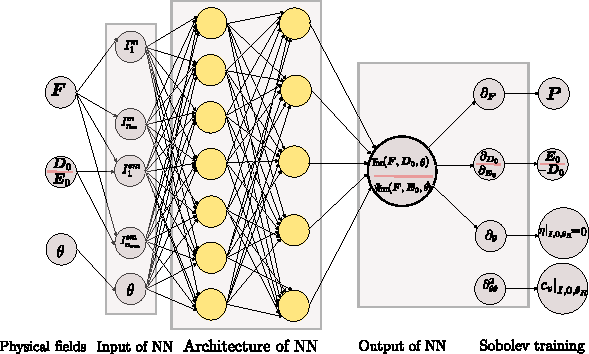
\includegraphics[width=0.85\textwidth]{Figures/InkScape/NN_2}
	\vspace{-2mm}
	\caption{Simplified structure of the neural network architecture used for calibration of the $\theta$-based network-based surrogate potentials i.e. $\Psi_{nn}$, $\Upsilon_{nn}$, for the case of Sobolev-type training strategy 2 in Section \ref{sec:strategy 2 theta}.}
	\label{fig:strategy 2}
\end{figure}




\newpage

\subsubsection{Mathematical formulation of the strategy: potentials depending upon $\eta$}\label{sec:strategy 2 eta}


For the two $\eta$-based potentials, specifically $e(\vect{F}, \vect{D}_0, \eta)$ and $\Gamma(\vect{F}, \vect{E}_0, \eta)$, the second calibration strategy introduces a distinct differentiation compared to the $\theta$-based potentials discussed in Section \ref{sec:strategy 2 theta}. The key distinction lies in the fact that one of the inputs to these potentials, the entropy $\eta$, is not directly available from the given data. Instead, what is provided is the temperature, which corresponds to the derivative of both potentials with respect to $\eta$. Consequently, $\eta$ must be determined implicitly through the nonlinear relationships presented in the third column of the first and third rows of equation \eqref{eqn:piola alternative}. This relationship can be mathematically reformulated as:
%
\begin{equation}\label{eqn:thermo}
\begin{aligned}
&\text{Given } \{\vect{F},\vect{D}_0,\theta\}\, \text{, solve } \eta \text{ from:            }\theta   =  \partial_{\eta}e_{nn}(\vect{F},\vect{D}_0,\eta)\\
%
&\text{Given } \{\vect{F},\vect{E}_0,\theta\}\, \text{, solve } \eta \text{ from:            }\theta   =  \partial_{\eta}\Gamma_{nn}(\vect{F},\vect{E}_0,\eta)
\end{aligned}
\end{equation}




For these entropy-based dependent potentials, i.e.  $e_{nn}(\vect{F},\vect{D}_0,\theta,\vect{\mathcal{W}})$ and $\Gamma_{nn}(\vect{F},\vect{E}_0,\theta,\vect{\mathcal{W}})$, this  alternative and more physically oriented calibration approach,  the specific objective is to satisfy the implicit relationship in \eqref{eqn:thermo} whilst minimizing the discrepancy between: 
%
\begin{itemize}

	
	%
	\item  \(
	e_{nn}\left\{
	\begin{aligned}
	&\text{the derivatives }  \{\partial_{\vect{F}}e_{nn},\partial_{\vect{D}_0}e_{nn},\partial_{\eta}e_{nn}\} \text{ and } \{\vect{P},\vect{E}_0,\theta\}:=\{\partial_{\vect{F}}\Psi,{\vect{E}_0},\theta\}\\
	%
	&\text{the field } \frac{\theta}{\partial^2_{\theta\theta} e} \text{ and } c_v:=-\theta\Psi^2_{\theta\theta}\\
	%
	&\{\vect{F},\vect{D}_0\} \text{ are data }\\
	& \eta \text{ is not data and it is obtained implicitly from } \theta = \partial_{\eta}e_{nn}(\vect{F},\vect{D}_0,\eta)	 
	\end{aligned}
	\right.
	\)
	
	%

	
	\item  \(	\Gamma_{nn}\left\{
	\begin{aligned}
	&\text{the derivatives }   \{\partial_{\vect{F}}\Gamma_{nn},-\partial_{\vect{E}_0}\Gamma_{nn},\partial_{\eta}\Gamma_{nn}\} \text{ and } \{\vect{P},\vect{D}_0,\theta\}:=\{\partial_{\vect{F}}\Psi,-\partial_{\vect{E}_0}\Psi,\theta\}\\
	%
	&\text{the field } \frac{\theta}{\partial^2_{\theta\theta} \Gamma} \text{ and } c_v:=-\theta\Psi^2_{\theta\theta}\\
	%
	&\{\vect{F},\vect{D}_0\} \text{ are data }\\
	& \eta \text{ is not data and it is obtained implicitly from } \theta = \partial_{\eta}\Gamma_{nn}(\vect{F},\vect{E}_0,\eta)	 		
	\end{aligned}
	\right.
	\)	
	
	
	
	
\end{itemize}
%


A second distinguishing feature of the second calibration approach applied to $\eta$-based potentials again arises from the fact that one of the inputs, specifically $\eta$, is not directly available from the data set. In particular, when solving, for example, using a Newton-Raphson numerical scheme to iteratively resolve equation \eqref{eqn:thermo}, certain convexity and stability conditions must be satisfied to ensure the existence of a solution. These conditions are inherently embedded within equation \eqref{eqn:rank one convexity other potentials}, necessitating the convexity of both potentials $e_{nn}$ and $\Gamma_{nn}$ with respect to $\eta$, namely:
%
\begin{equation}\label{eqn:convexity}
\partial^2_{\eta\eta}e_{nn}(\vect{F},\vect{D}_0,\eta)>0;\qquad \partial^2_{\eta\eta} \Gamma_{nn}(\vect{F},\vect{E}_0,\eta)>0
\end{equation}

We found that the numerical solution of \eqref{eqn:thermo} benefits from the imposition of the condition in the reference confuguration in equation \ref{eqn:reference conditions for the different potentials}, namely
%
\begin{equation}\label{eqn:reference eta}
\left.\partial_{\eta}e(\vect{F},\vect{D}_0,\eta)\right\vert_{\vect{I},\vect{0},0}  =  \theta_R;\qquad 
\left.\partial_{\eta}\Gamma(\vect{F},\vect{E}_0,\eta)\right\vert_{\vect{I},\vect{0},0}  =  \theta_R
\end{equation}

To inherently satisfy both conditions \eqref{eqn:reference eta} and \eqref{eqn:convexity} within the neural network-based potentials $e_{nn}$ and $\Gamma_{nn}$, we propose the formulation of modified potentials, denoted as $\widetilde{e}_{nn}$ and $\widetilde{\Gamma}_{nn}$.
%
\begin{equation}\label{eqn:modified potentials}
\begin{aligned}
&\widetilde{e}_{nn}(\vect{F},\vect{D}_0,\eta) =  \underbrace{{e}_{nn}(\vect{F},\vect{D}_0,\eta)}_{\text{Neural network model}} + \underbrace{\left(\theta_R-\left.\partial_{\eta}{e}_{nn}(\vect{F},\vect{D}_0,\eta)\right\vert_{\vect{I},\vect{0},0}\right)\eta}_{\text{Condition enforcement in reference conf.}} + \underbrace{\alpha_{\text{stb}}\frac{\theta_R}{2{c_v}_R}\eta^2}_{\text{Stabilizing term}}\\
%
&\widetilde{\Gamma}_{nn}(\vect{F},\vect{E}_0,\eta) =  \underbrace{{\Gamma}_{nn}(\vect{F},\vect{E}_0,\eta)}_{\text{Neural network model}} + \underbrace{\left(\theta_R-\left.\partial_{\eta}{\Gamma}_{nn}(\vect{F},\vect{D}_0,\eta)\right\vert_{\vect{I},\vect{0},0}\right)\eta}_{\text{Condition enforcement in reference conf.}} + \underbrace{\alpha_{\text{stb}}\frac{\theta_R}{2{c_v}_R}\eta^2}_{\text{Stabilizing term}}
%
\end{aligned}
\end{equation}

In fact, evaluation of the first and second derivative with respect to $\eta$ for both modified potentials in \eqref{eqn:modified potentials} yields

\begin{equation}\label{eqn:conditions imposed}
\begin{aligned}
&\partial_{\eta}\Rightarrow\left\{\begin{aligned}
\partial_{\eta}\widetilde{e}_{nn}(\vect{F},\vect{D}_0,\eta) &=  \partial_{\eta}{e}_{nn}(\vect{F},\vect{D}_0,\eta) + \theta_R-\left.\partial_{\eta}{e}_{nn}(\vect{F},\vect{D}_0,\eta)\right\vert_{\vect{I},\vect{0},0} + \alpha_{\text{stb}}\frac{\theta_R}{{c_v}_R}\eta\\
%
%
\partial_{\eta}\widetilde{\Gamma}_{nn}(\vect{F},\vect{E}_0,\eta) &=  \partial_{\eta}{\Gamma}_{nn}(\vect{F},\vect{E}_0,\eta) + \theta_R-\left.\partial_{\eta}{\Gamma}_{nn}(\vect{F},\vect{E}_0,\eta)\right\vert_{\vect{I},\vect{0},0} + \alpha_{\text{stb}}\frac{\theta_R}{{c_v}_R}\eta\end{aligned}\right.\\
%
%
&\partial^2_{\eta\eta}\Rightarrow\left\{\begin{aligned}
\partial^2_{\eta\eta}\widetilde{e}_{nn}(\vect{F},\vect{D}_0,\eta)& =  \partial^2_{\eta\eta}{e}_{nn}(\vect{F},\vect{D}_0,\eta)+ \underbrace{\alpha_{\text{stb}}\frac{\theta_R}{{c_v}_R}}_{>0}\\
%
\partial^2_{\eta\eta}\widetilde{\Gamma}_{nn}(\vect{F},\vect{E}_0,\eta)& =  \partial^2_{\eta\eta}{\Gamma}_{nn}(\vect{F},\vect{E}_0,\eta)+ \underbrace{\alpha_{\text{stb}}\frac{\theta_R}{{c_v}_R}}_{>0}
%
\end{aligned}\right.
\end{aligned}
\end{equation}


Clearly, evaluation of the first derivative in \eqref{eqn:conditions imposed} in the reference configuration for both potentials leads to the satisfaction of the condition in equation \eqref{eqn:reference eta}, namely
%
\begin{equation}
\begin{aligned}
\left.\partial_{\eta}\widetilde{e}_{nn}(\vect{F},\vect{D}_0,\eta)\right\vert_{\vect{I},\vect{0},0}& =  \left.\partial_{\eta}{e}_{nn}(\vect{F},\vect{D}_0,\eta)\right\vert_{\vect{I},\vect{0},0} + \theta_R-\left.\partial_{\eta}{e}_{nn}(\vect{F},\vect{D}_0,\eta)\right\vert_{\vect{I},\vect{0},0} = \theta_R\\
%
\left.\partial_{\eta}\widetilde{\Gamma}_{nn}(\vect{F},\vect{E}_0,\eta)\right\vert_{\vect{I},\vect{0},0} &=  \left.\partial_{\eta}{\Gamma}_{nn}(\vect{F},\vect{E}_0,\eta)\right\vert_{\vect{I},\vect{0},0} + \theta_R-\left.\partial_{\eta}{\Gamma}_{nn}(\vect{F},\vect{E}_0,\eta)\right\vert_{\vect{I},\vect{0},0} = \theta_R
\end{aligned}
%
\end{equation}


To examine the second derivative in \eqref{eqn:conditions imposed}, it becomes evident that while the second term is positive, there is no guarantee that the overall derivative, specifically $\partial^2_{\eta\eta}\widetilde{e}_{nn}(\vect{F},\vect{D}0,\eta)$ and $\partial^2_{\eta\eta}\widetilde{\Gamma}_{nn}(\vect{F},\vect{E}0,\eta)$, will be positive. The positivity of these derivatives is contingent upon the chosen value of the stabilizing parameter $\alpha{\text{stb}}$. Based on our empirical observations, we have determined that setting $\alpha_{\text{stb}} = 0.25$ suffices to prevent numerical instabilities during the solution of equation \eqref{eqn:thermo}.

The calibration method for the $\eta$-based potentials outlined above is depicted schematically in Figure \ref{fig:strategy 2 eta}. To achieve the primary goal of this calibration approach, we define the associated Sobolev-type loss functions, with their specific formulations detailed in Table \ref{table: sobolev type 2 eta}.







\begin{table}[htbp!]
	\centering
	\begin{tabular}{c c c}
		\toprule
		\rowcolor{gray!30}	\small{} & $\mathcal{L}(\vect{\mathcal{W}})$ &\\
		\midrule
		%
		$e_{nn}$	&	\begin{minipage}{0.65\textwidth}
			\begin{equation*}
			\begin{aligned}
			& \beta_1\frac{\sum_{i=1}^{n_{\text{d}}} \vert\vert \partial_{\vect{F}}\Psi^{i} - \partial_{\vect{F}} e_{nn}(\vect{X}^i, \vect{\mathcal{W}}) \vert\vert^2}{\sum_{i=1}^{n_{\text{d}}} \vert\vert \partial_{\vect{F}}\Psi^{i} \vert\vert^2}  + \beta_2\frac{\sum_{i=1}^{n_{\text{d}}} \vert\vert \vect{E}_0^{i} - \partial_{\vect{D}_0} e_{nn}(\vect{X}^i, \vect{\mathcal{W}}) \vert\vert^2}{\sum_{i=1}^{n_{\text{d}}} \vert\vert \vect{E}_0^{i} \vert\vert^2} \\
			& + \beta_3\frac{\sum_{i=1}^{n_{\text{d}}} \Big( \theta^{i} - \partial_{\eta} e_{nn}(\vect{X}^i, \vect{\mathcal{W}})\Big)^2 }{\sum_{i=1}^{n_{\text{d}}}  \left(\theta^{i}\right)^2 }
			\end{aligned}
			\end{equation*}
		\end{minipage}  & $\vect{X}^i=\{\vect{F}^i, -\partial_{\vect{E}_0}\Psi^i, -\partial_{\theta}\Psi^i\}$ 	\\
		%
		%
		%
		$\Gamma_{nn}$	&	\begin{minipage}{0.68\textwidth}
			\begin{equation*}
			\begin{aligned}
			& \beta_1\frac{\sum_{i=1}^{n_{\text{d}}} \vert\vert \partial_{\vect{F}}\Psi^{i} - \partial_{\vect{F}} \Gamma_{nn}(\vect{X}^i, \vect{\mathcal{W}}) \vert\vert^2}{\sum_{i=1}^{n_{\text{d}}} \vert\vert\partial_{\vect{F}}\Psi^{i} \vert\vert^2}  + \beta_2\frac{\sum_{i=1}^{n_{\text{d}}} \vert\vert \partial_{\vect{E}_0}\Psi^{i} - \partial_{\vect{E}_0} \Gamma_{nn}(\vect{X}^i, \vect{\mathcal{W}}) \vert\vert^2}{\sum_{i=1}^{n_{\text{d}}} \vert\vert \partial_{\vect{E}_0}\Psi^{i} \vert\vert^2} \\
			& + \beta_3\frac{\sum_{i=1}^{n_{\text{d}}} \left( \theta^{i} - \partial_{\eta} \Gamma_{nn}(\vect{X}^i, \vect{\mathcal{W}}) \right)^2}{\sum_{i=1}^{n_{\text{d}}} \left( \theta^{i} \right)^2}
			\end{aligned}
			\end{equation*}
		\end{minipage} & $\vect{X}^i=\{\vect{F}^i, \vect{E}_0^i, -\partial_{\theta}\Psi^i\}$	\\
		\midrule
		
		
		%
	\end{tabular}
	\caption{Loss functions $\mathcal{L}(\vect{\mathcal{W}})$ used for the calibration of $\eta$-based neural network-based surrogate potentials, i.e. $e_{nn}$,  $\Gamma_{nn}$, for the case of Sobolev-type training strategy 2 described in Section \ref{sec:strategy 2 eta}. All the potentials have been calibrated with data obtained from Helmholtz free energy density ground truth models, i.e. $\Psi$. The index $i$ represents in-silico data number $i$, and $n_d$ the number of data used for calibration, whereas $n_{c_v}$ represents the number of data used for the measurement/evaluation of $c_v$.}
	\label{table: sobolev type 2 eta}
\end{table}




\begin{figure}[htpb!]
	\centering
	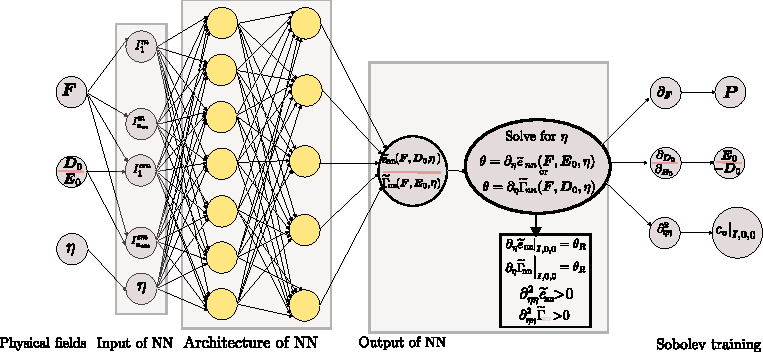
\includegraphics[width=1.0\textwidth]{Figures/InkScape/NN_3}
	\vspace{-2mm}
	\caption{Simplified structure of the neural network architecture used for calibration of the $\eta$-based network-based surrogate potentials i.e. $e_{nn}$, $\Gamma_{nn}$, for the case of Sobolev-type training strategy 2 in Section \ref{sec:strategy 2 eta}. Enforcement of conditions \eqref{eqn:convexity} and \eqref{eqn:reference eta} is carried out through the modifications in equation \eqref{eqn:modified potentials}.}
	\label{fig:strategy 2 eta}
\end{figure}


\subsubsection{In-silico data generation strategy}

In this section, we briefly described the procedure used for generating synthetic data for the calibration strategy denoted as strategy 2. The procedure is entirely the same as for strategy 1, summarised in Algorithm \ref{alg:sample_generation}. The generation of deformation gradient tensors (step 1 in Algorithm \ref{alg:sample_generation}) and electric fields $\vect{E}_0$ or electric displacement fields $\vect{D}_0$ (step 2 in Algorithm \ref{alg:sample_generation}) is entirely the same as for strategy 1 in Algorithm \ref{alg:sample_generation}. The main difference lies with regards step 3 in Algorithm \ref{alg:sample_generation}. We summarise for convenience the steps followed in the data generation procedure for calibration strategy 1, and supplement those for calibration strategy 2, permitting a direct comparison between both strategies:

\vspace{2mm}

\noindent{\textbf{Data generation strategy 1:}}
\vspace{-2mm}
\begin{itemize}
	\item For $\theta$-based potentials, i.e. $\Psi_{nn}(\vect{F},\vect{E}_0,\theta)$ or $\Upsilon_{nn}(\vect{F},\vect{D}_0,\theta)$, fields $\{\vect{F},\vect{E}_0,\theta\}$ or $\{\vect{F},\vect{D}_0,\theta\}$, respectively, are generated as input data according to Algorithm \ref{alg:sample_generation}. Evaluation of the model permits then to synthetically generate the work conjugate fields $\{\vect{P},\vect{D}_0,\eta\}$ or $\{\vect{P},\vect{E}_0,\eta\}$, respectively, as output variables. 
	
	\item For $\eta$-based potentials, i.e. $e(\vect{F},\vect{D}_0,\eta)$ and $\Gamma(\vect{F},\vect{E}_0,\eta)$, the process is the opposite:  $\{\vect{F},\vect{D}_0,\eta\}$ or $\{\vect{F},\vect{E}_0,\eta\}$, respectively, are generated as input data according to Algorithm \ref{alg:sample_generation}. Evaluation of the model permits then to synthetically generate the work conjugate fields $\{\vect{P},\vect{E}_0,\theta\}$ or $\{\vect{P},\vect{D}_0,\theta\}$, respectively, as output variables.	
\end{itemize} 


\vspace{2mm}

\noindent{\textbf{Data generation strategy 2:}}
\vspace{-2mm}

\begin{itemize}
	\item For $\theta$-based potentials, i.e. $\Psi_{nn}(\vect{F},\vect{E}_0,\theta)$ or $\Upsilon_{nn}(\vect{F},\vect{D}_0,\theta)$, data for fields $\{\vect{F},\vect{E}_0,\theta\}$ or $\{\vect{F},\vect{D}_0,\theta\}$, respectively, are generated as input data according to Algorithm \ref{alg:sample_generation}. Then, the fields $\{\vect{P},\vect{D}_0\}$ or $\{\vect{P},\vect{E}_0\}$ (generated as synthetic data through direct evaluation of the analytical model or through experiments), respectively, are considered as output variables. The entropy field $\eta$ is discarded (for synthetic approaches) or directly not available (for experimental procedures). In addition, data for the specific heat capacity $c_v$ is needed (see Section \ref{sec:strategy 2 theta}).
	
	\item For $\eta$-based potentials, i.e. $e(\vect{F},\vect{D}_0,\eta)$ and $\Gamma(\vect{F},\vect{E}_0,\eta)$, data for fields $\{\vect{F},\vect{D}_0,\theta\}$ or $\{\vect{F},\vect{E}_0,\theta\}$, respectively, are generated according to Algorithm \ref{alg:sample_generation}.  Out of the three fields, only two $\{\vect{F},\vect{D}_0\}$ or $\{\vect{F},\vect{D}_0\}$, respectively, are considered to be input variables. The third field, namely $\theta$, is used to solve implicitly the entropy field $\eta$ according to \eqref{eqn:thermo}. Then, the fields  $\{\vect{P},\vect{D}_0\}$ or $\{\vect{P},\vect{E}_0\}$ (generated as synthetic data through direct evaluation of the analytical model or through experiments), respectively, are considered as output variables in conjunction with $\theta$. In addition, data for the specific heat capacity $c_v$ is needed (see Section \ref{sec:strategy 2 theta}).
\end{itemize} 



